%% 
%% Copyright 2007, 2008, 2009 Elsevier Ltd
%% 
%% This file is part of the 'Elsarticle Bundle'.
%% ---------------------------------------------
%% 
%% It may be distributed under the conditions of the LaTeX Project Public
%% License, either version 1.2 of this license or (at your option) any
%% later version.  The latest version of this license is in
%%    http://www.latex-project.org/lppl.txt
%% and version 1.2 or later is part of all distributions of LaTeX
%% version 1999/12/01 or later.
%% 
%% The list of all files belonging to the 'Elsarticle Bundle' is
%% given in the file `manifest.txt'.
%% 
%% Template article for Elsevier's document class `elsarticle'
%% with harvard style bibliographic references
%% SP 2008/03/01

\documentclass[preprint,12pt,authoryear]{elsarticle}

%% Use the option review to obtain double line spacing
%% \documentclass[authoryear,preprint,review,12pt]{elsarticle}

%% Use the options 1p,twocolumn; 3p; 3p,twocolumn; 5p; or 5p,twocolumn
%% for a journal layout:
%% \documentclass[final,1p,times,authoryear]{elsarticle}
%% \documentclass[final,1p,times,twocolumn,authoryear]{elsarticle}
%% \documentclass[final,3p,times,authoryear]{elsarticle}
%% \documentclass[final,3p,times,twocolumn,authoryear]{elsarticle}
%% \documentclass[final,5p,times,authoryear]{elsarticle}
%% \documentclass[final,5p,times,twocolumn,authoryear]{elsarticle}

\usepackage[T1]{fontenc}
\usepackage[utf8]{inputenc}

%% For including figures, graphicx.sty has been loaded in
%% elsarticle.cls. If you prefer to use the old commands
%% please give \usepackage{epsfig}

%% The amssymb package provides various useful mathematical symbols
\usepackage{amssymb}
%% The amsthm package provides extended theorem environments
\usepackage{amsthm}

%% The lineno packages adds line numbers. Start line numbering with
%% \begin{linenumbers}, end it with \end{linenumbers}. Or switch it on
%% for the whole article with \linenumbers.
%% \usepackage{lineno}

\journal{Neucocomputing}

%%% Adding metadata:
\newsubfloat{figure}
\newsubfloat{table}
% Better page layout for A4 paper, see memoir manual.
\settrimmedsize{297mm}{210mm}{*}
\setlength{\trimtop}{0pt} 
\setlength{\trimedge}{\stockwidth} 
\addtolength{\trimedge}{-\paperwidth} 
\settypeblocksize{634pt}{448.13pt}{*} 
\setulmargins{4cm}{*}{*} 
\setlrmargins{*}{*}{1.5} 
\setmarginnotes{17pt}{51pt}{\onelineskip} 
\setheadfoot{\onelineskip}{2\onelineskip} 
\setheaderspaces{*}{2\onelineskip}{*} 
\checkandfixthelayout
%
\frenchspacing
% Font with math support: New Century Schoolbook
\usepackage{fouriernc}
\usepackage[T1]{fontenc}
%
% UoB guidelines:
%
% Text should be in double or 1.5 line spacing, and font size should be
% chosen to ensure clarity and legibility for the main text and for any
% quotations and footnotes. Margins should allow for eventual hard binding.
%
% Note: This is automatically set by memoir class. Nevertheless \OnehalfSpacing 
% enables double spacing but leaves single spaced for captions for instance. 
\OnehalfSpacing 
%
% Sets numbering division level
\setsecnumdepth{subsection} 
\maxsecnumdepth{subsubsection}
%
% Chapter style (taken and slightly modified from Lars Madsen Memoir Chapter 
% Styles document
\usepackage{calc,soul,fourier}

\iffalse
\makeatletter 
\newlength\dlf@normtxtw 
\setlength\dlf@normtxtw{\textwidth} 
\newsavebox{\feline@chapter} 
\newcommand\feline@chapter@marker[1][4cm]{%
	\sbox\feline@chapter{% 
		\resizebox{!}{#1}{\fboxsep=1pt%
			\colorbox{gray}{\color{white}\thechapter}% 
		}}%
		\rotatebox{90}{% 
			\resizebox{%
				\heightof{\usebox{\feline@chapter}}+\depthof{\usebox{\feline@chapter}}}% 
			{!}{\scshape\so\@chapapp}}\quad%
		\raisebox{\depthof{\usebox{\feline@chapter}}}{\usebox{\feline@chapter}}%
} 
\newcommand\feline@chm[1][4cm]{%
	\sbox\feline@chapter{\feline@chapter@marker[#1]}% 
	\makebox[0pt][c]{% aka \rlap
		\makebox[1cm][r]{\usebox\feline@chapter}%
	}}
\makechapterstyle{daleifmodif}{
	\renewcommand\chapnamefont{\normalfont\Large\scshape\raggedleft\so} 
	\renewcommand\chaptitlefont{\normalfont\Large\bfseries\scshape} 
	\renewcommand\chapternamenum{} \renewcommand\printchaptername{} 
	\renewcommand\printchapternum{\null\hfill\feline@chm[2.5cm]\par} 
	\renewcommand\afterchapternum{\par\vskip\midchapskip} 
	\renewcommand\printchaptertitle[1]{\color{gray}\chaptitlefont\raggedleft ##1\par}
} 
\makeatother 
\chapterstyle{daleifmodif}
\fi
%
% UoB guidelines:
%
% The pages should be numbered consecutively at the bottom centre of the
% page.
\makepagestyle{myvf} 
\makeoddfoot{myvf}{}{\thepage}{} 
\makeevenfoot{myvf}{}{\thepage}{} 
\makeheadrule{myvf}{\textwidth}{\normalrulethickness} 
\makeevenhead{myvf}{\small\textsc{\leftmark}}{}{} 
\makeoddhead{myvf}{}{}{\small\textsc{\rightmark}}
\pagestyle{myvf}
%
% Oscar's command (it works):
% Fills blank pages until next odd-numbered page. Used to emulate single-sided
% frontmatter. This will work for title, abstract and declaration. Though the
% contents sections will each start on an odd-numbered page they will
% spill over onto the even-numbered pages if extending beyond one page
% (hopefully, this is ok).
\newcommand{\clearemptydoublepage}{\newpage{\thispagestyle{empty}\cleardoublepage}}
%
%
% Creates indexes for Table of Contents, List of Figures, List of Tables and Index
\makeindex
% \printglossaries below creates a list of abbreviations. \gls and related
% commands are then used throughout the text, so that latex can automatically
% keep track of which abbreviations have already been defined in the text.
%
% The import command enables each chapter tex file to use relative paths when
% accessing supplementary files. For example, to include
% chapters/brewing/images/figure1.png from chapters/brewing/brewing.tex we can
% use
% \includegraphics{images/figure1}
% instead of
% \includegraphics{chapters/brewing/images/figure1}
\usepackage{import}

% Add other packages needed for chapters here. For example:
\usepackage{lipsum}					%Needed to create dummy text
\usepackage{amsfonts} 					%Calls Amer. Math. Soc. (AMS) fonts
\usepackage[centertags]{amsmath}			%Writes maths centred down
\usepackage{stmaryrd}					%New AMS symbols
\usepackage{amssymb}					%Calls AMS symbols
\usepackage{amsthm}					%Calls AMS theorem environment
\usepackage{newlfont}					%Helpful package for fonts and symbols
\usepackage{layouts}					%Layout diagrams
\usepackage{graphicx}					%Calls figure environment
\usepackage{longtable,rotating}			%Long tab environments including rotation. 
\usepackage[utf8]{inputenc}			%Needed to encode non-english characters 
									%directly for mac
\usepackage{colortbl}					%Makes coloured tables
\usepackage{wasysym}					%More math symbols
\usepackage{mathrsfs}					%Even more math symbols
\usepackage{float}						%Helps to place figures, tables, etc. 
\usepackage{verbatim}					%Permits pre-formated text insertion
\usepackage{upgreek }					%Calls other kind of greek alphabet
\usepackage{latexsym}					%Extra symbols
\usepackage[square,numbers,
		     sort&compress]{natbib}		%Calls bibliography commands 
\usepackage{url}						%Supports url commands
\usepackage{etex}						%eTeXÕs extended support for counters
\usepackage{fixltx2e}					%Eliminates some in felicities of the 
									%original LaTeX kernel
\usepackage[spanish,english]{babel}		%For languages characters and hyphenation
\usepackage{color}                    				%Creates coloured text and background
\usepackage[colorlinks=true,
		     allcolors=black]{hyperref}              %Creates hyperlinks in cross references
\usepackage{memhfixc}					%Must be used on memoir document 
									%class after hyperref
\usepackage{enumerate}					%For enumeration counter
\usepackage{footnote}					%For footnotes
\usepackage{microtype}					%Makes pdf look better.
\usepackage{rotfloat}					%For rotating and float environments as tables, 
									%figures, etc. 
\usepackage{alltt}						%LaTeX commands are not disabled in 
									%verbatim-like environment
\usepackage[version=0.96]{pgf}			%PGF/TikZ is a tandem of languages for producing vector graphics from a 
\usepackage{tikz}						%geometric/algebraic description.
\usetikzlibrary{arrows,shapes,snakes,
		       automata,backgrounds,
		       petri,topaths}				%To use diverse features from tikz		
%							
%Reduce widows  (the last line of a paragraph at the start of a page) and orphans 
% (the first line of paragraph at the end of a page)
\widowpenalty=1000
\clubpenalty=1000
%
% New command definitions for my thesis
%

\newcommand{\keywords}[1]{\par\noindent{\small{\bf Keywords:} #1}} %Defines keywords small section
\newcommand{\parcial}[2]{\frac{\partial#1}{\partial#2}}                             %Defines a partial operator
\newcommand{\vectorr}[1]{\mathbf{#1}}                                                        %Defines a bold vector
\newcommand{\vecol}[2]{\left(                                                                         %Defines a column vector
	\begin{array}{c} 
		\displaystyle#1 \\
		\displaystyle#2
	\end{array}\right)}
\newcommand{\mados}[4]{\left(                                                                       %Defines a 2x2 matrix
	\begin{array}{cc}
		\displaystyle#1 &\displaystyle #2 \\
		\displaystyle#3 & \displaystyle#4
	\end{array}\right)}
\newcommand{\pgftextcircled}[1]{                                                                    %Defines encircled text
    \setbox0=\hbox{#1}%
    \dimen0\wd0%
    \divide\dimen0 by 2%
    \begin{tikzpicture}[baseline=(a.base)]%
        \useasboundingbox (-\the\dimen0,0pt) rectangle (\the\dimen0,1pt);
        \node[circle,draw,outer sep=0pt,inner sep=0.1ex] (a) {#1};
    \end{tikzpicture}
}
\newcommand{\range}[1]{\textnormal{range }#1}                                             %Defines range operator
\newcommand{\innerp}[2]{\left\langle#1,#2\right\rangle}                                 %Defines inner product
\newcommand{\prom}[1]{\left\langle#1\right\rangle}                                         %Defines average operator
\newcommand{\tra}[1]{\textnormal{tra} \: #1}                                                       %Defines trace operator
\newcommand{\sign}[1]{\textnormal{sign\,}#1}                                                   %Defines sign operator
\newcommand{\sech}[1]{\textnormal{sech} #1}                                                  %Defines sech
\newcommand{\diag}[1]{\textnormal{diag} #1}                                                    %Defines diag operator
\newcommand{\arcsech}[1]{\textnormal{arcsech} #1}                                       %Defines arcsech
\newcommand{\arctanh}[1]{\textnormal{arctanh} #1}                                         %Defines arctanh
%Change tombstone symbol
\newcommand{\blackged}{\hfill$\blacksquare$}
\newcommand{\whiteged}{\hfill$\square$}
\newcounter{proofcount}
\renewenvironment{proof}[1][\proofname.]{\par
 \ifnum \theproofcount>0 \pushQED{\whiteged} \else \pushQED{\blackged} \fi%
 \refstepcounter{proofcount}
 \normalfont 
 \trivlist
 \item[\hskip\labelsep
       \itshape
   {\bf\em #1}]\ignorespaces
}{%
 \addtocounter{proofcount}{-1}
 \popQED\endtrivlist
}
%
%
% New definition of square root:
% it renames \sqrt as \oldsqrt
\let\oldsqrt\sqrt
% it defines the new \sqrt in terms of the old one
\def\sqrt{\mathpalette\DHLhksqrt}
\def\DHLhksqrt#1#2{%
\setbox0=\hbox{$#1\oldsqrt{#2\,}$}\dimen0=\ht0
\advance\dimen0-0.2\ht0
\setbox2=\hbox{\vrule height\ht0 depth -\dimen0}%
{\box0\lower0.4pt\box2}}
%
% My caption style
\newcommand{\mycaption}[2][\@empty]{
	\captionnamefont{\scshape} 
	\changecaptionwidth
	\captionwidth{0.9\linewidth}
	\captiondelim{.\:} 
	\indentcaption{0.75cm}
	\captionstyle[\centering]{}
	\setlength{\belowcaptionskip}{10pt}
	\ifx \@empty#1 \caption{#2}\else \caption[#1]{#2}
}
%
% My subcaption style
\newcommand{\mysubcaption}[2][\@empty]{
	\subcaptionsize{\small}
	\hangsubcaption
	\subcaptionlabelfont{\rmfamily}
	\sidecapstyle{\raggedright}
	\setlength{\belowcaptionskip}{10pt}
	\ifx \@empty#1 \subcaption{#2}\else \subcaption[#1]{#2}
}
%
%An initial of the very first character of the content
\usepackage{lettrine}
\newcommand{\initial}[1]{%
	\lettrine[lines=3,lhang=0.33,nindent=0em]{
		\color{gray}
     		{\textsc{#1}}}{}}
%
% Theorem styles used in my thesis
%
\theoremstyle{plain}
\newtheorem{theo}{Theorem}[chapter]
\theoremstyle{plain}
\newtheorem{prop}{Proposition}[chapter]
\theoremstyle{plain}
\theoremstyle{definition}
\newtheorem{dfn}{Definition}[chapter]
\theoremstyle{plain}
\newtheorem{lema}{Lemma}[chapter]
\theoremstyle{plain}
\newtheorem{cor}{Corollary}[chapter]
\theoremstyle{plain}
\newtheorem{resu}{Result}[chapter]
\theoremstyle{plain}
\newtheorem{algo}{Algorithm}[chapter]
\theoremstyle{plain}
\newtheorem{assu}{Assumption}[chapter]
%
% Hyphenation for some words
%
\hyphenation{res-pec-tively}
\hyphenation{mono-ti-ca-lly}
\hyphenation{hypo-the-sis}
\hyphenation{para-me-ters}
\hyphenation{sol-va-bi-li-ty}
%
%
%%\newcommand{\Rd}{\mathbb{R}^d}  	
\newcommand{\hy}{\hat{y}_t}
\newcommand{\hY}{\hat{Y}_t}
\newcommand{\ty}{\tilde{y}_t}		
\newcommand{\xt}{\mathbf{x}_t}
\newcommand{\indicator}{\mathds{1}_{(\hy\neq y_t)}}
\newcommand{\0}{\mathds{0}}
\newcommand{\1}{\mathds{1}}
\newcommand{\2}{\mathds{2}}
\newcommand{\3}{\mathds{3}}
\newcommand{\4}{\mathds{4}}
\newcommand{\5}{\mathds{5}}
\newcommand{\6}{\mathds{6}}
\newcommand{\7}{\mathds{7}}
\newcommand{\8}{\mathds{8}}
\newcommand{\9}{\mathds{9}}
\newcommand{\RKd}{\mathbb{R}^{K\times d}}
\newcommand{\ARMSET}{\mathscr{A}}
\newcommand{\inspace}{\mathscr{X}}
\newcommand{\outspace}{\mathscr{Y}}
\newcommand{\pxy}{\Phi(\mathbf{x},y)}
\newcommand{\argmaxi}{\underset{i\in \{1,\dots,K\}}{\text{argmax}}}
\newcommand{\instance}{\mathbf{x}_t,y_t}
\newcommand{\examples}{(\mathbf{x}_1,y_1),\dots,(\mathbf{x}_T,y_T)}
\newcommand{\sumk}{\sum_{k=1}^{K}}
\newcommand{\sumd}{\sum_{i=1}^{d}}
\newcommand{\sumt}{\sum_{t=1}^{T}}
\newcommand{\loss}{\mathscr{l}}
\newcommand{\cumuloss}{\mathscr{L}}
\newcommand{\labels}{\mathbf{L}}
\newcommand{\E}{\mathbb{E}}
\newcommand{\tY}{\tilde{Y}_t}
\newcommand{\inputS}{\mathscr{X}}
\newcommand{\outputS}{\mathscr{Y}}
\newcommand{\Ut}{\tau_t \sum_{k=1}^{K}(2\beta_t^k-1)\Phi(x_t,k)}
\newcommand{\p}{\mathbf{p}}
\newcommand{\Prob}{\mathbf{P}}
\newcommand{\bfx}{\mathbf{x}}
\newcommand{\bfy}{\mathbb{y}}
\newcommand{\R}{\mathbb{R}}
\newcommand{\ep}{\epsilon}
\newcommand{\epPF}{\mathscr{A}_{\epsilon}^{\ast}}
\newcommand{\hp}{\hat{p}}
\newcommand{\pp}{\mathbb{P}}

\begin{document}

\begin{frontmatter}

%% Title, authors and addresses

%% use the tnoteref command within \title for footnotes;
%% use the tnotetext command for theassociated footnote;
%% use the fnref command within \author or \address for footnotes;
%% use the fntext command for theassociated footnote;
%% use the corref command within \author for corresponding author footnotes;
%% use the cortext command for theassociated footnote;
%% use the ead command for the email address,
%% and the form \ead[url] for the home page:
%% \title{Title\tnoteref{label1}}
%% \tnotetext[label1]{}
%% \author{Name\corref{cor1}\fnref{label2}}
%% \ead{email address}
%% \ead[url]{home page}
%% \fntext[label2]{}
%% \cortext[cor1]{}
%% \address{Address\fnref{label3}}
%% \fntext[label3]{}

\title{The title}

%% use optional labels to link authors explicitly to addresses:
%% \author[label1,label2]{}
%% \address[label1]{}
%% \address[label2]{}

\author[centrale,lif]{Hongliang Zhong}
\author[centrale,ins]{Emmanuel Dauc\'e \corref{cor1}}

\address[centrale]{Ecole Centrale de Marseille}
\address[lif]{Laboratoire d'informatique Fondamentale}
\address[ins]{Institut de Neurosciences des Syst\`emes}

\cortext[cor1]{Corresponding author}

\begin{abstract}
%% Text of abstract

\end{abstract}

\begin{keyword}
%% keywords here, in the form: keyword \sep keyword
Mot1 \sep Mot2
%% PACS codes here, in the form: \PACS code \sep code

%% MSC codes here, in the form: \MSC code \sep code
%% or \MSC[2008] code \sep code (2000 is the default)

\end{keyword}

\end{frontmatter}

%% \linenumbers

%% main text
\section{Introduction}
\label{sec:intro}

\paragraph{Bandit with side information}




\section{Models}

\section{Analysis}

\section{Experiments}

\subsection{High-dimensional datassets}
\label{subsec:BPAE}
Here, we evaluate the algorithms over two synthetic and three real world data sets. Their characteristics are summarized in Table~\ref{table:mce}.

\begin{table}[h]
	\caption{Summary of the three high-dimensional datasets, including the numbers of instances, features, labels and whether the number of examples in each class are balanced.}
	\label{table:mce}
	\begin{center}
		\begin{tabular}{l l l l l}
			{\bf Dataset}  & {\bf Instances} & {\bf Features} & {\bf Labels}& {\bf Balanced}\\
			\hline
			SynSep & $10^5$ 	& 400 	& 9 & Y\\
			
			SynNonSep & $10^5$ & 400 	& 9 & Y\\
			
			RCV1-v2  & $10^5$ 	& 47236 	& 53 & N\\
			
			%Letter 	&$2*10^4$	&16	&26	&N\\
			
			%Pen-Based &$1.32*10^4$	&16	&10	&N\\
		\end{tabular}
	\end{center}
\end{table}

\textbf{Data sets}:
The first data set, denoted by SynSep,  is a 9-class, 400-dimensional synthetic data set of size $10^5$. More details about the method to generate this data set can be found in \cite{kakade2008efficient}. The SynSep  idea is to have a simple simulation of generating a text document. The coordinates represent different words in a small vocabulary of size $400$. We ensure that SynSep is linearly separable. 

The second data set, denoted by SynNonSep, is constructed  the same way as  SynSep except that a 5\% label noise is introduced, which makes the data set non-separable. 

The third data set is collected from the Reuters RCV1-v2 collection\cite{David04RCV}. The original data set is composed by multi-label instances. So we make some preprocessing likes \cite{RB08a}. First, its label hierarchy is reorganized by mapping the data set to the second level of RCV1 topic hierarchy. The documents that have labels of the third or forth level only are mapped to their parent category of the second level; Second, all multi-labelled instances have been removed. This RCV1-v2 is a 53-class,  47236-dimensional real data set of size $10^5$. 

%The fourth and fifth data sets are collected from \cite{letter26SC,number10SC}. The fourth data set is to identify each of a large number of black-and-white rectangular pixel displays as one of the 26 capital letters in the English alphabet. The character images were based on 20 different fonts and each letter within these 20 fonts was randomly distorted to produce a file of 20000 unique stimuli. Each stimuli was converted into 16 primitive numerical attributes (statistical moments and edge counts). It forms a 26-class, 16-dimensional real data set of size $20000$. The fifth data set is a digit data base made by collecting 250 samples from 44 writers, using only (x,y) coordinate information represented as constant length feature vectors, which were resampled to 8 points per digit (therefore the data set contains 8 points $\times$ 2 coordinates = 16 features). This one is a 10-class, 16-dimensional real data set of size $10992$.

\textbf{Results}
Figures \ref{pic:BPASS} and~\ref{pic:BPASNS} show the experimental results on two synthetic data sets. For SynSep, a separable linear data set, all algorithms except Banditron obtain a good performance; with the non-separable SynNonSep data, Confidit and BPA outperform the other algorithms, even the supervised algorithms.  To different datasets, the parameters of different algorithms refer to Table~\ref{table:bpa}.
\begin{table}[h]
	\caption{The summary of algorithm parameters for different datasets. P. denotes Perceptron, PA is Passive-Aggressive online algorithm, B. is Banditron, C. is Confidit and BPA.}
	\label{table:bpa}
	\begin{center}
		\begin{tabular}{lllllll}
			{\bf Dataset}  & {\bf P.} & {\bf PA } & {\bf B.}& {\bf C.} & {\bf BPA}\\
			\hline
			SynSep & null & $C=0$ & $\varepsilon = 0.014$ &$\eta = 10^3$ & $\varepsilon = 0.4,C = 0$\\
			
			SynNonSep & null & $C=10^{-2}$ & $\varepsilon =0.65$ & $\eta = 10^3$& $\varepsilon = 0.8,C = 10^{-2}$\\
			
			Reuters & null & $C=10^{-2}$ & $\varepsilon =0.4$ & $\eta = 10^2$ & $\varepsilon = 0.2,C = 10^{-2}$\\
			
			%LR(26 letters) & null &  $C=0.1$ & $\varepsilon = 0.2$& $\eta=10^2$ & $\varepsilon = 0.8,C= 1$ \\
			
			%LR(10 numbers) & null & $C=0.1$ & $\varepsilon= 0.4$& $\eta = 10$ & $\varepsilon = 0.6,C=1$\\
			
		\end{tabular}
	\end{center}
\end{table}

%\textcolor{red}{OK-- Il manque les valeurs des paramètres pour les différents algorithmes (faire un tableau comme dans la partie précédente).}

Figure~\ref{pic:BPARCV} %, ~\ref{pic:BPALR10} and~\ref{pic:BPALR26} 
presents the result on the real dataset. With this dataset, the supervised algorithms, despite their competitive advantage with respect to the ones with bandit feedback, do not significantly depart from BPA and Confidit, with classification results that clearly outperform Banditron. While having a lower computational complexity, BPA approach is even found to outperform Confidit in the most challenging situation, i.e. the high-dimensional case with a large number of classes (RCV1-v2 data set).

The $\epsilon$ parameter represents the exploration rate in Banditron and BPA algorithms. We compare on Figure 3 the average error rates obtained on the two algorithms for different values of $\epsilon$ on the different data sets. In contrast with Banditron, BPA shows that $\epsilon$ has a very little influence on the final error rate, indicating a capability to deal with small exploration rates.


\begin{figure}[h!]
	
	\centerline{
		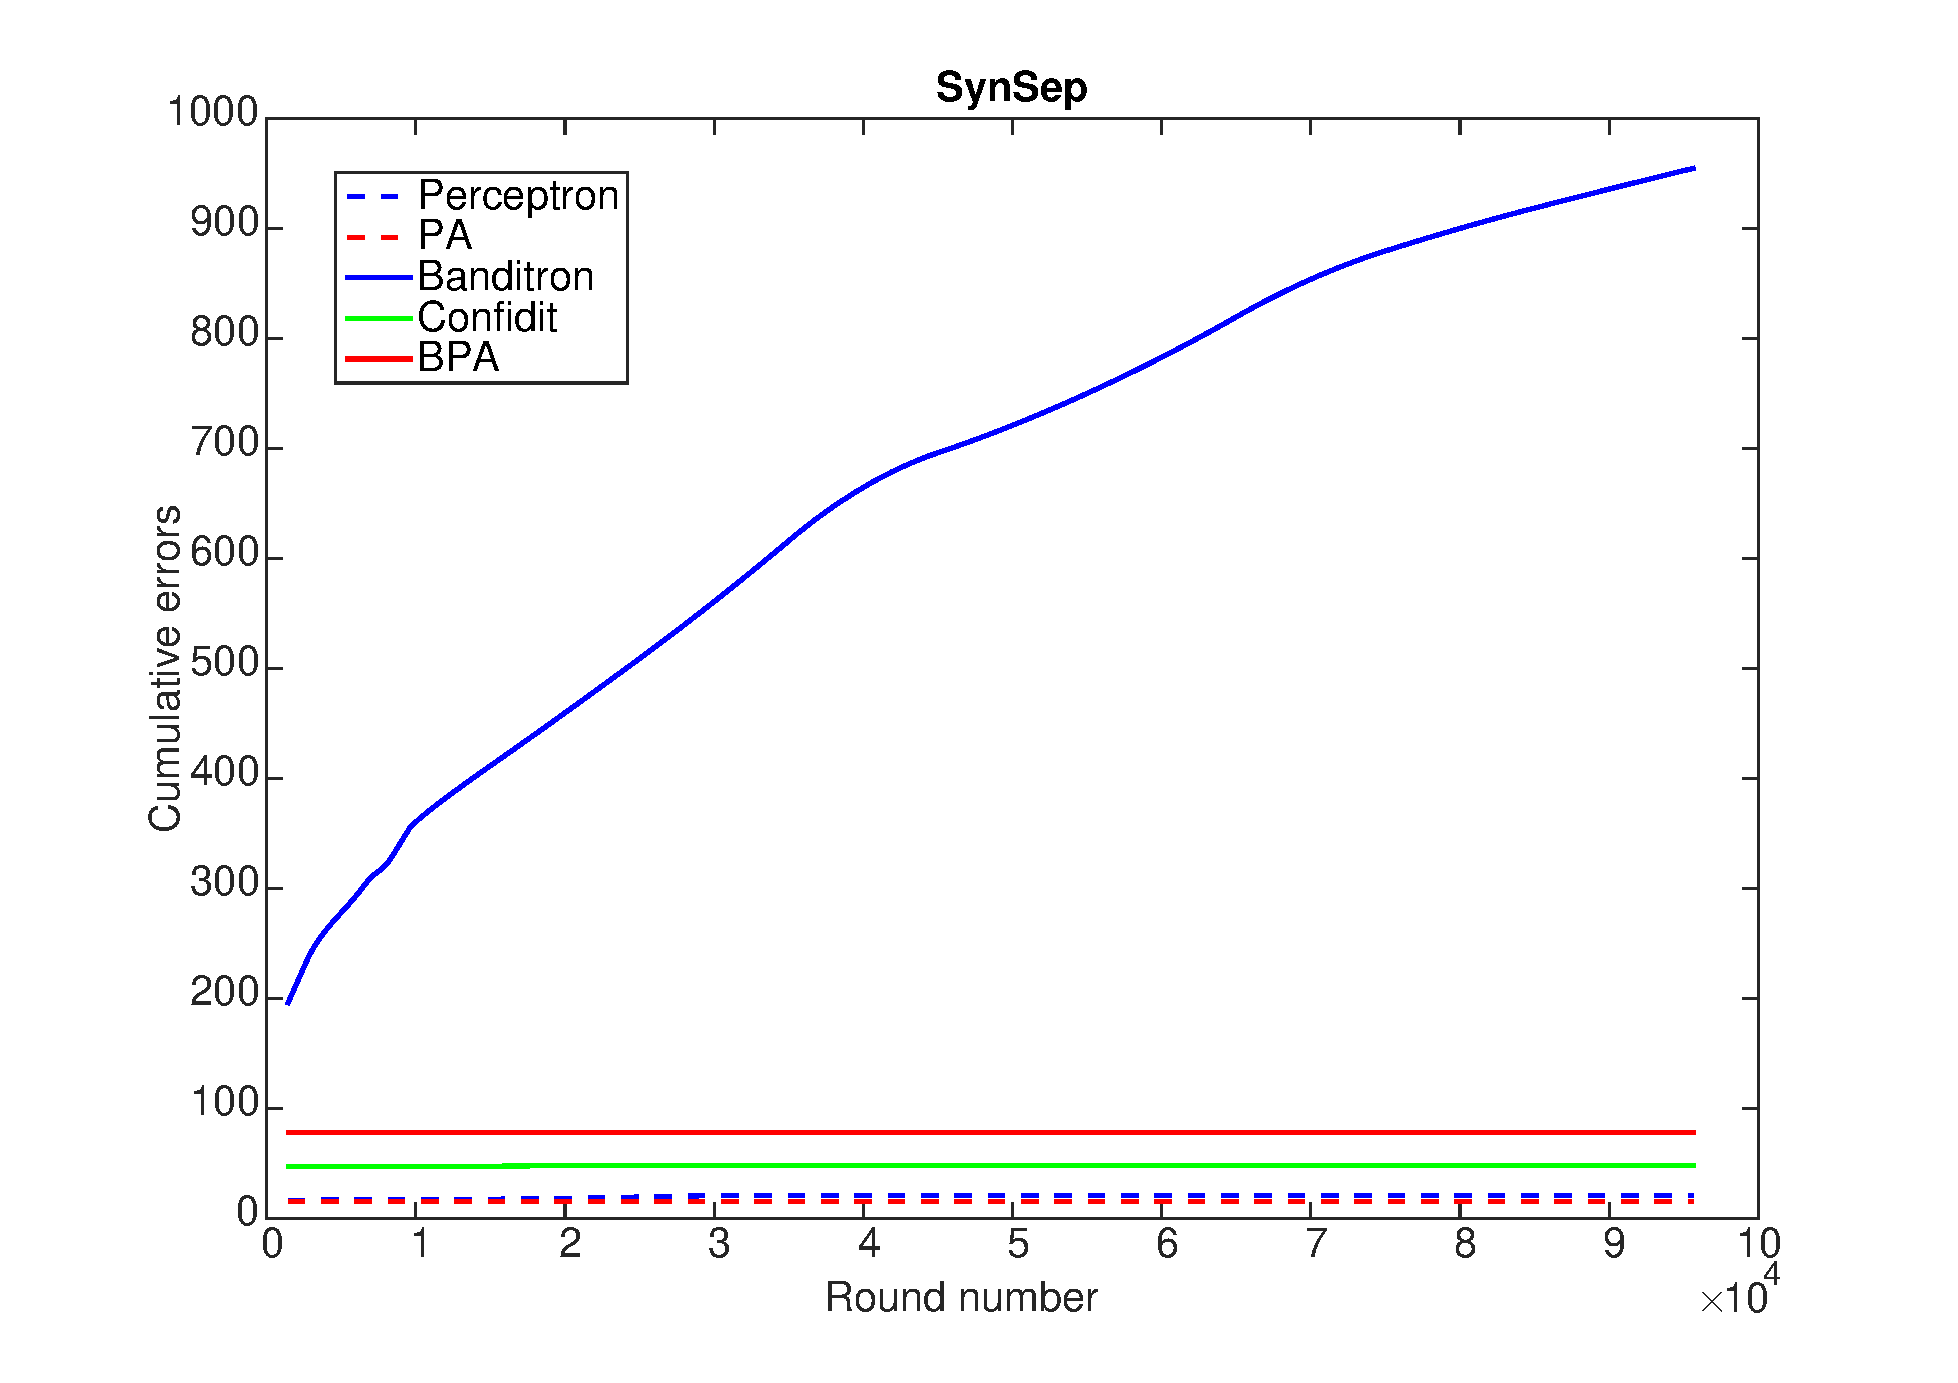
\includegraphics[scale = 0.4]{figs/SynSep.eps}
	}
	\caption{Cumulative Errors on the synthetic data set of  SynSep.}
	\label{pic:BPASS}
\end{figure}
\begin{figure}[h!]
	
	\centerline{
		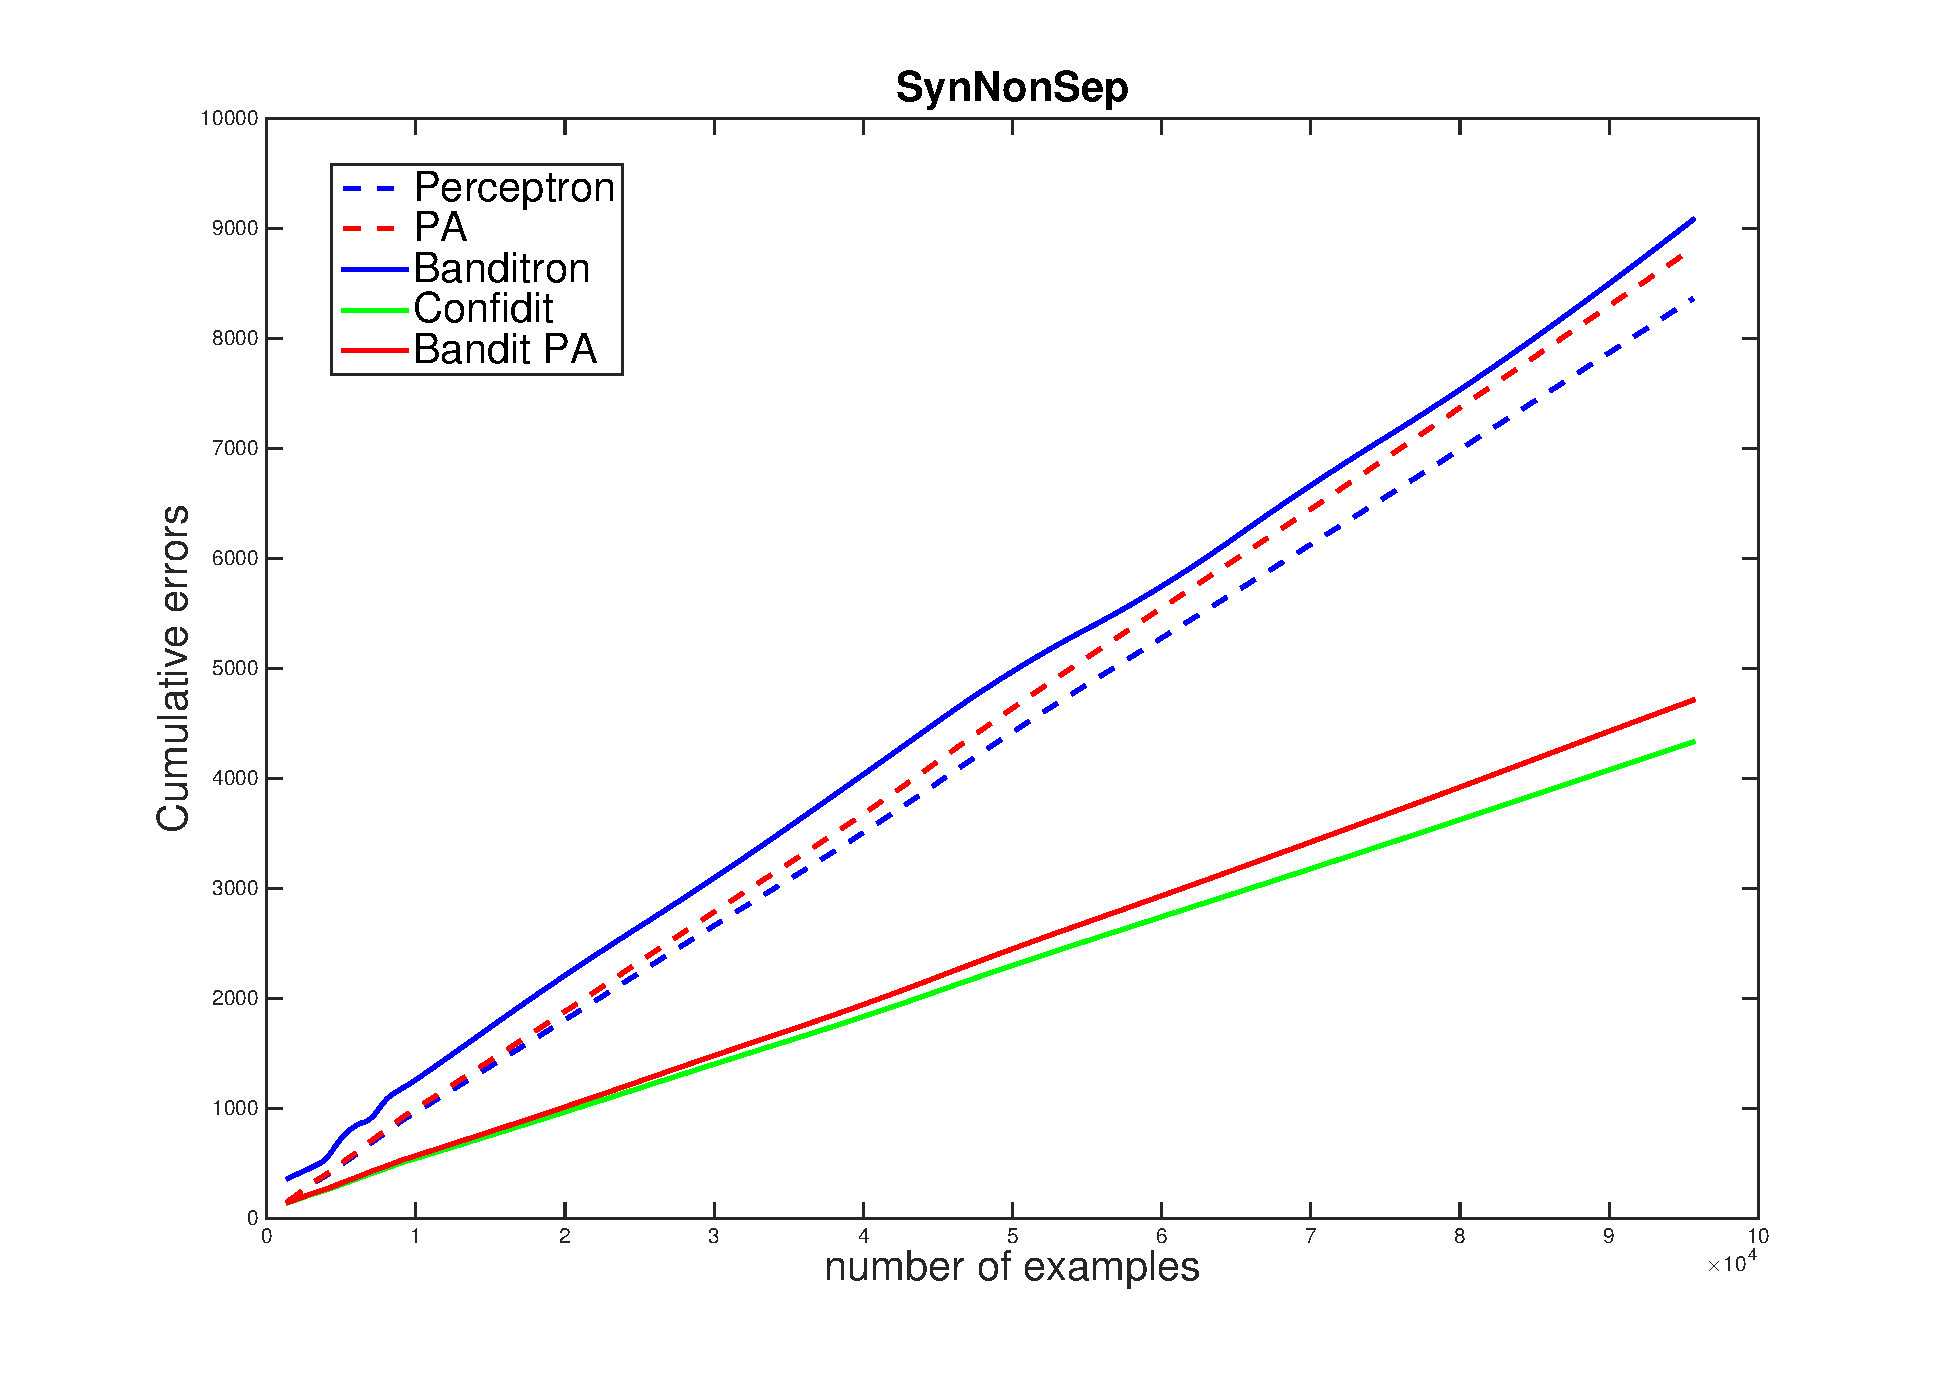
\includegraphics[scale = 0.4]{figs/SynNonSep.eps}
	}
	\caption{Cumulative Errors on the synthetic data set of SynNonSep.}
	\label{pic:BPASNS}
\end{figure}
\begin{figure}[h!]
	\centerline{
		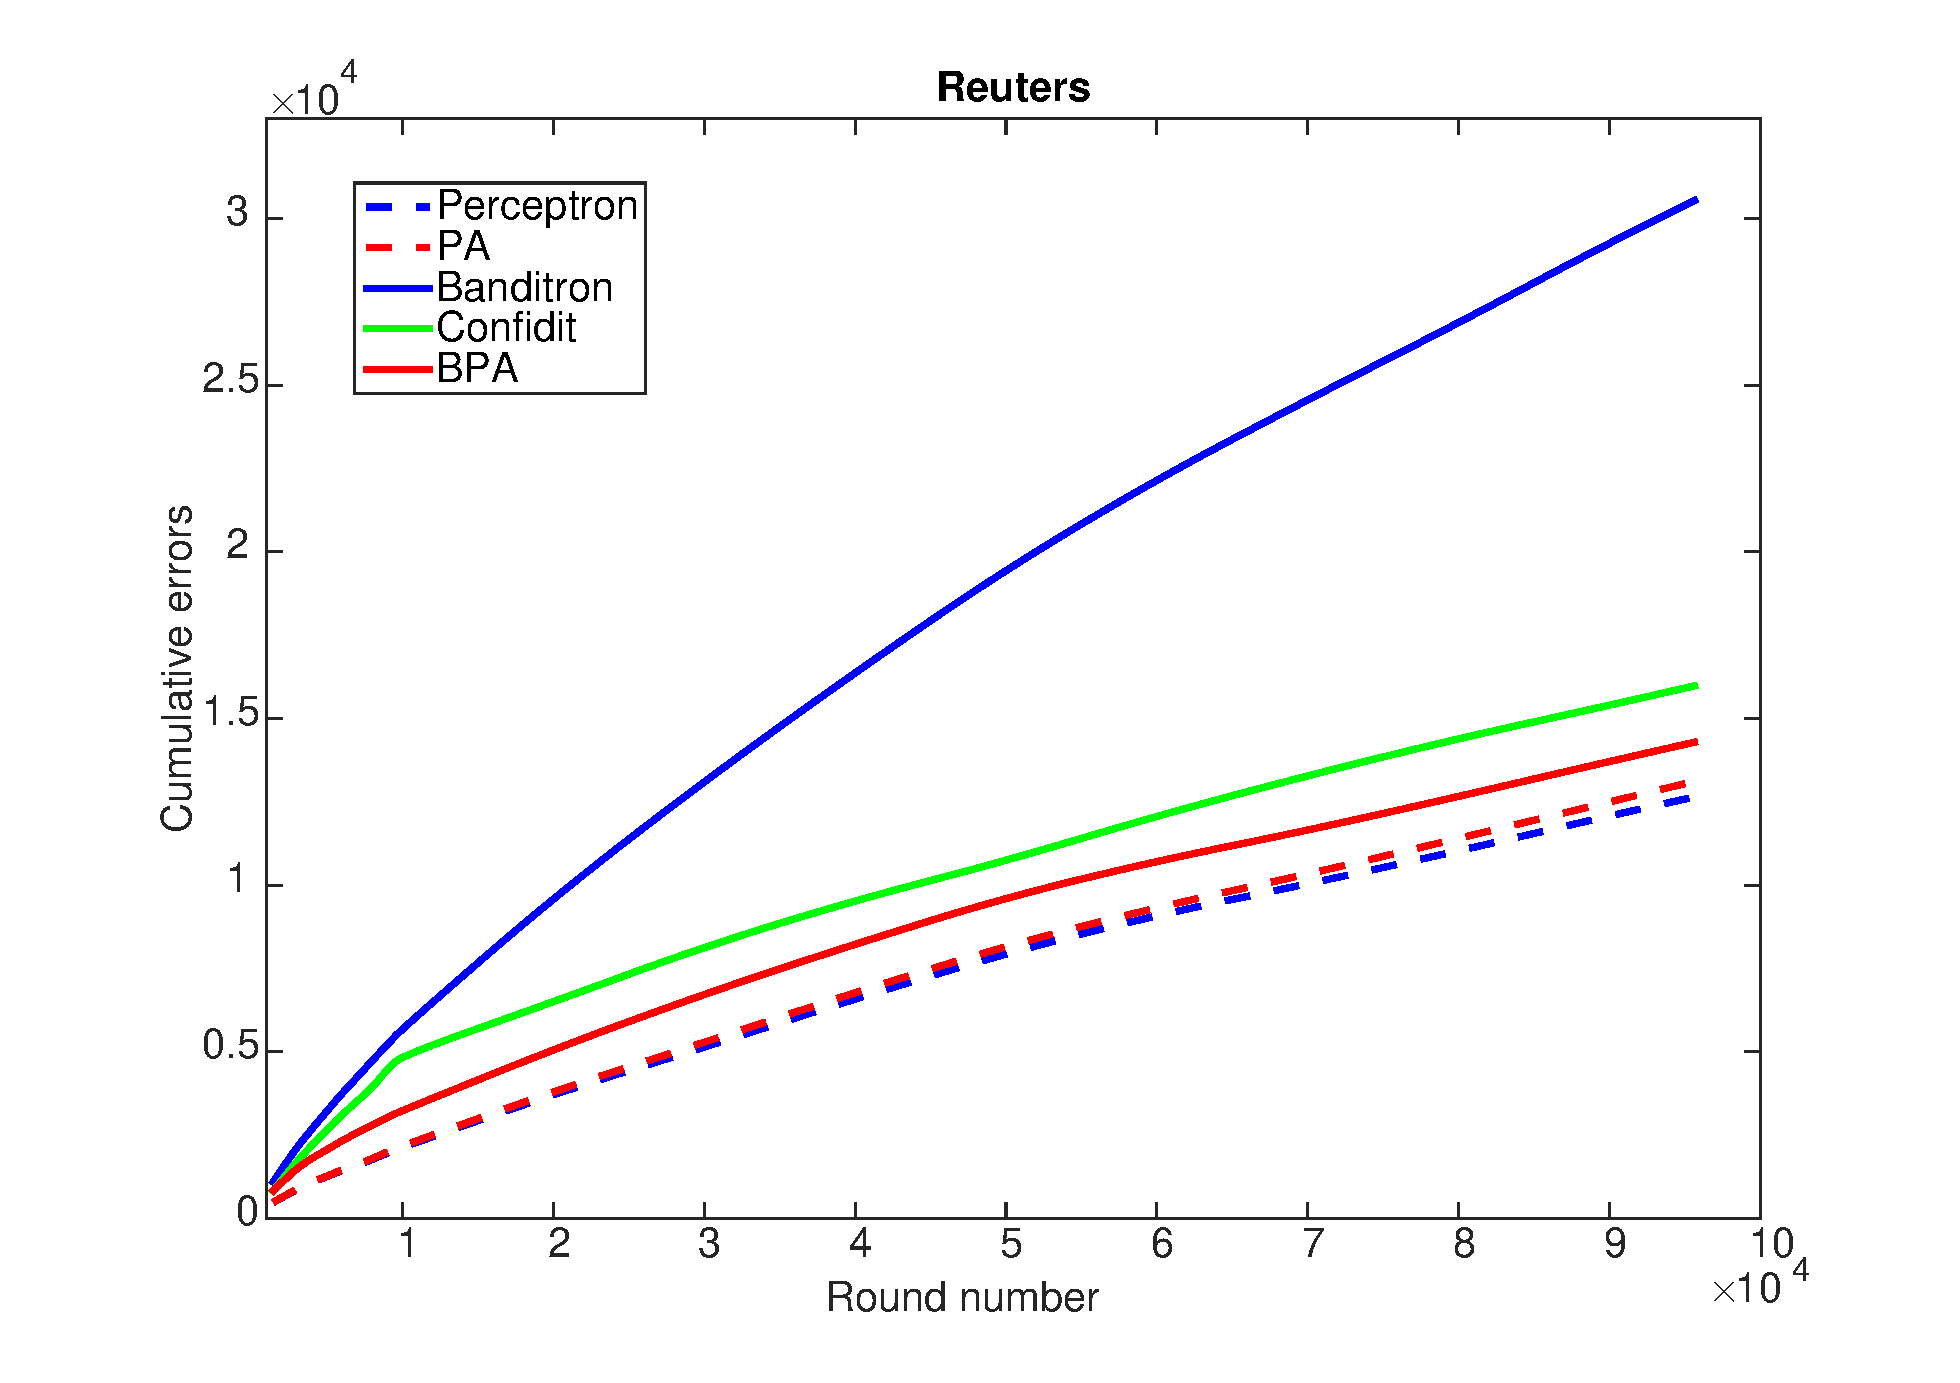
\includegraphics[scale = 0.4]{figs/RCV1_v2_53class.eps}}
	\caption{Cumulative Errors  on the real data set of RCV1-v2 (53 classes).}
	\label{pic:BPARCV}
\end{figure}

\begin{figure}[h!]
	\centerline{
		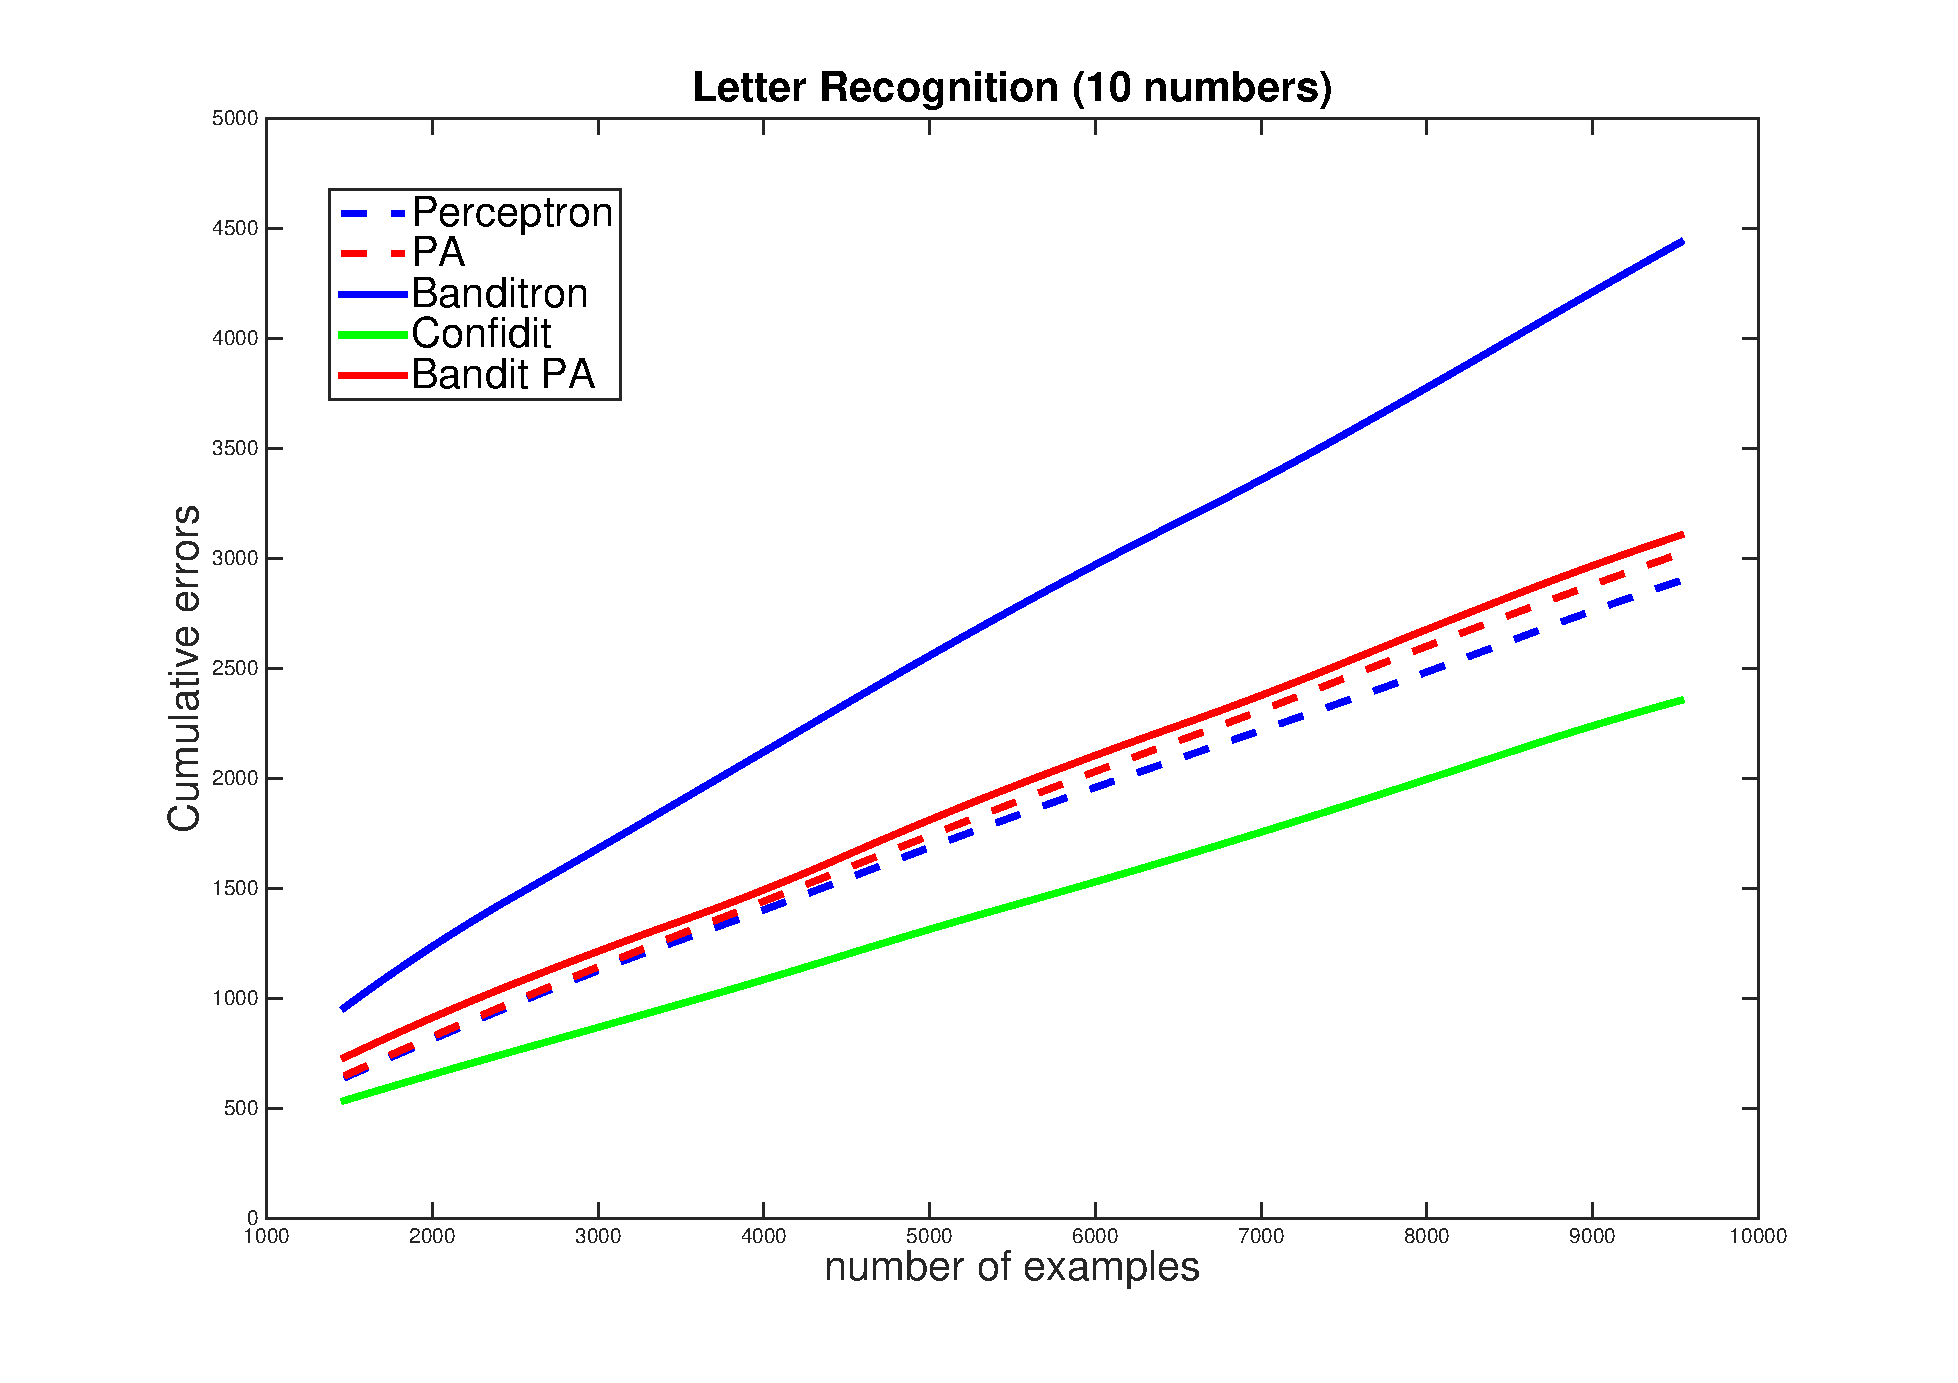
\includegraphics[scale = 0.4]{figs/10LR.eps}}
	\caption{Cumulative Errors on the real data set of Letter Recognition (10 numbers).}
	\label{pic:BPALR10}
\end{figure}

\begin{figure}[h!]
	\centerline{
		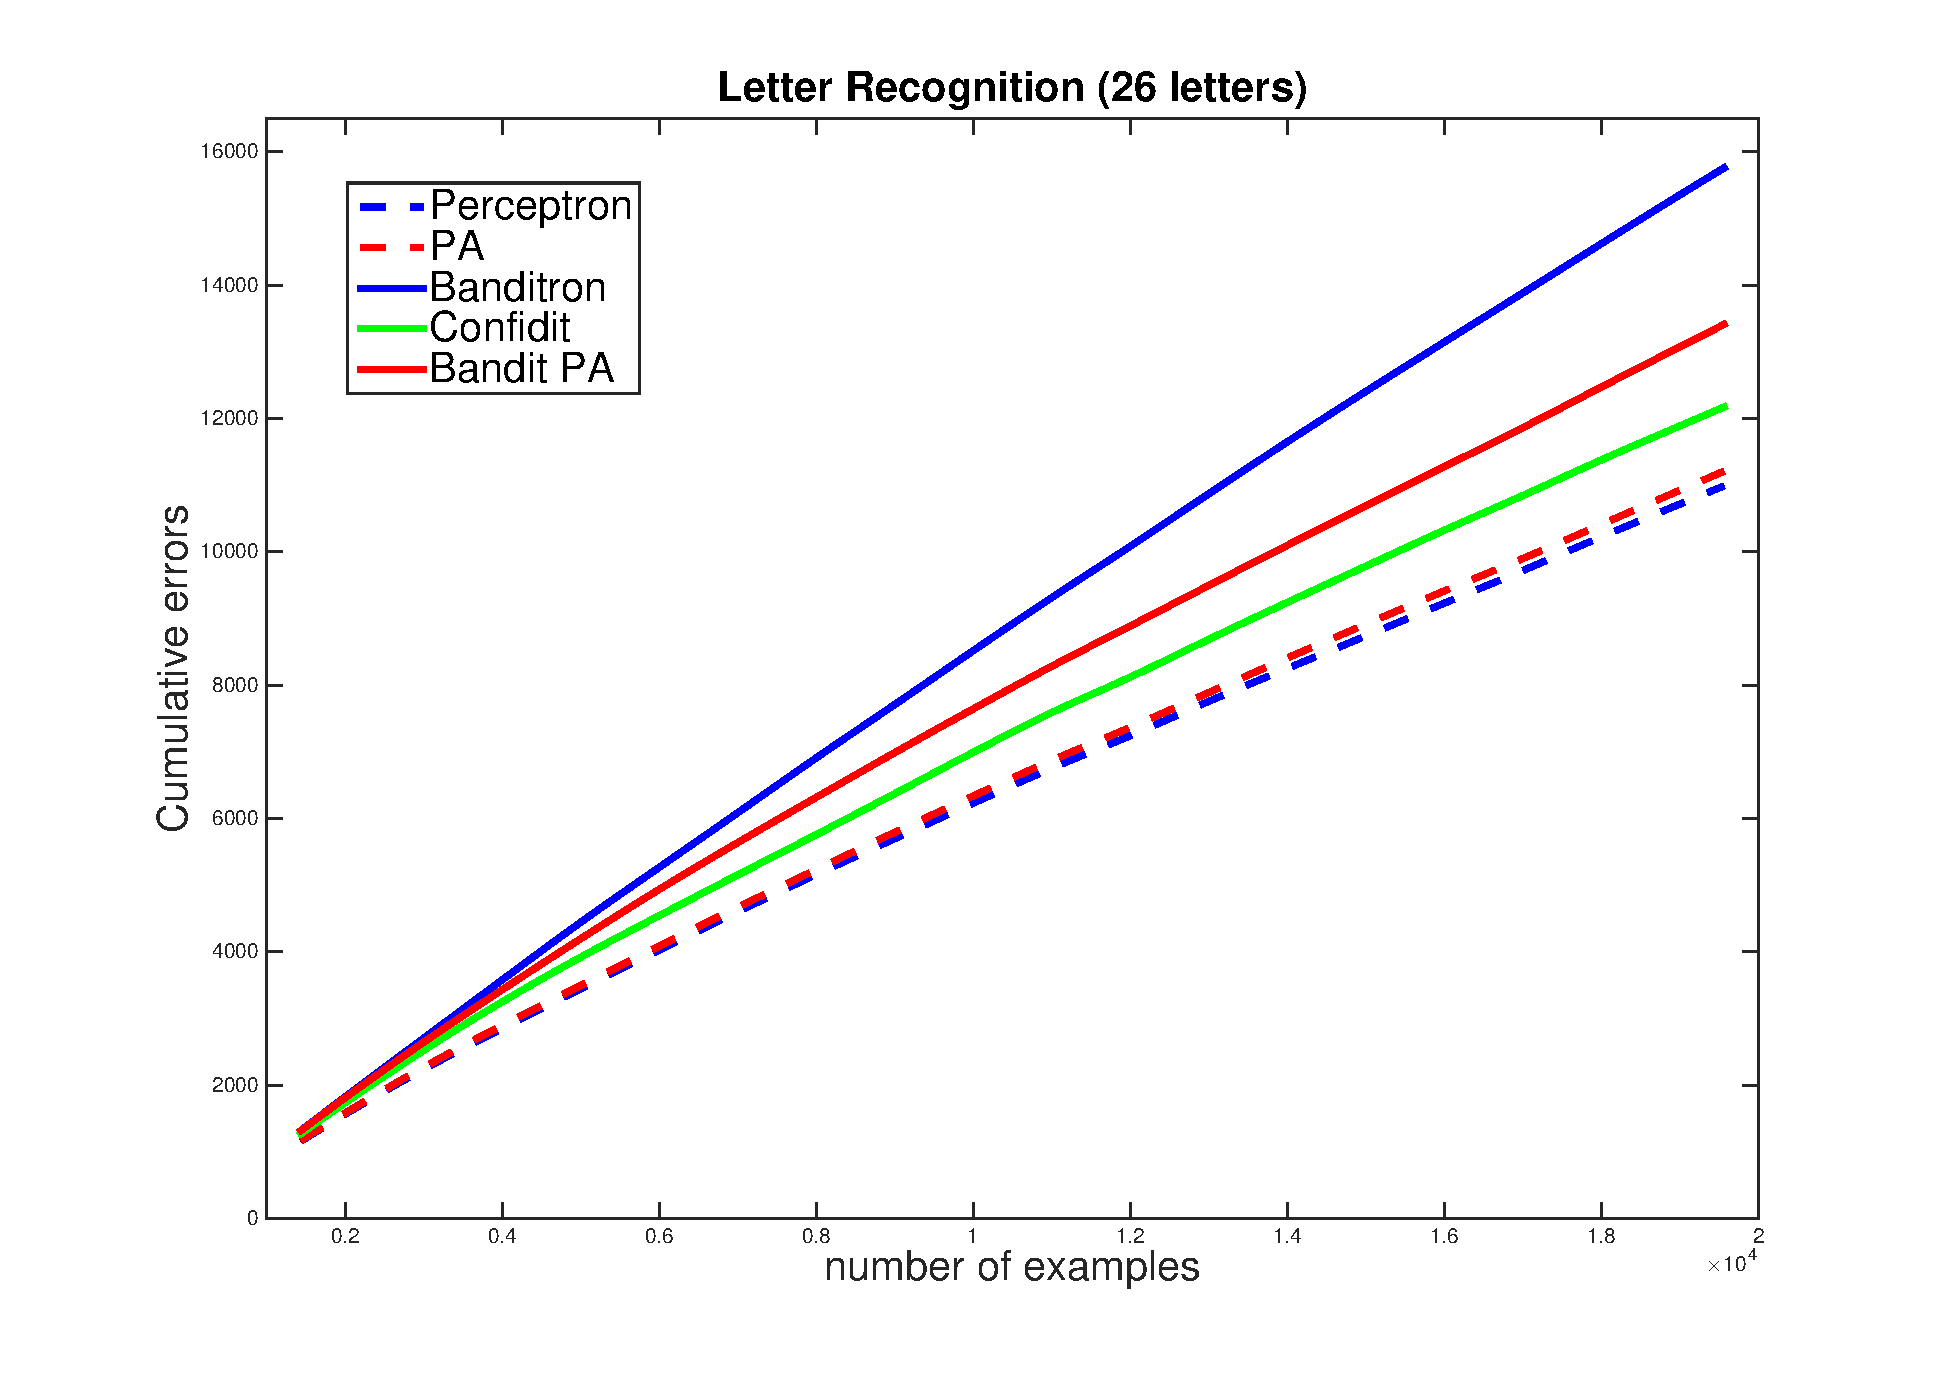
\includegraphics[scale = 0.4]{figs/26LR.eps}}
	\caption{Cumulative Errors  on the real data set of Letter Recognition (26 Letters).}
	\label{pic:BPALR26}
\end{figure}

\begin{figure}[h!]
	\centerline{
		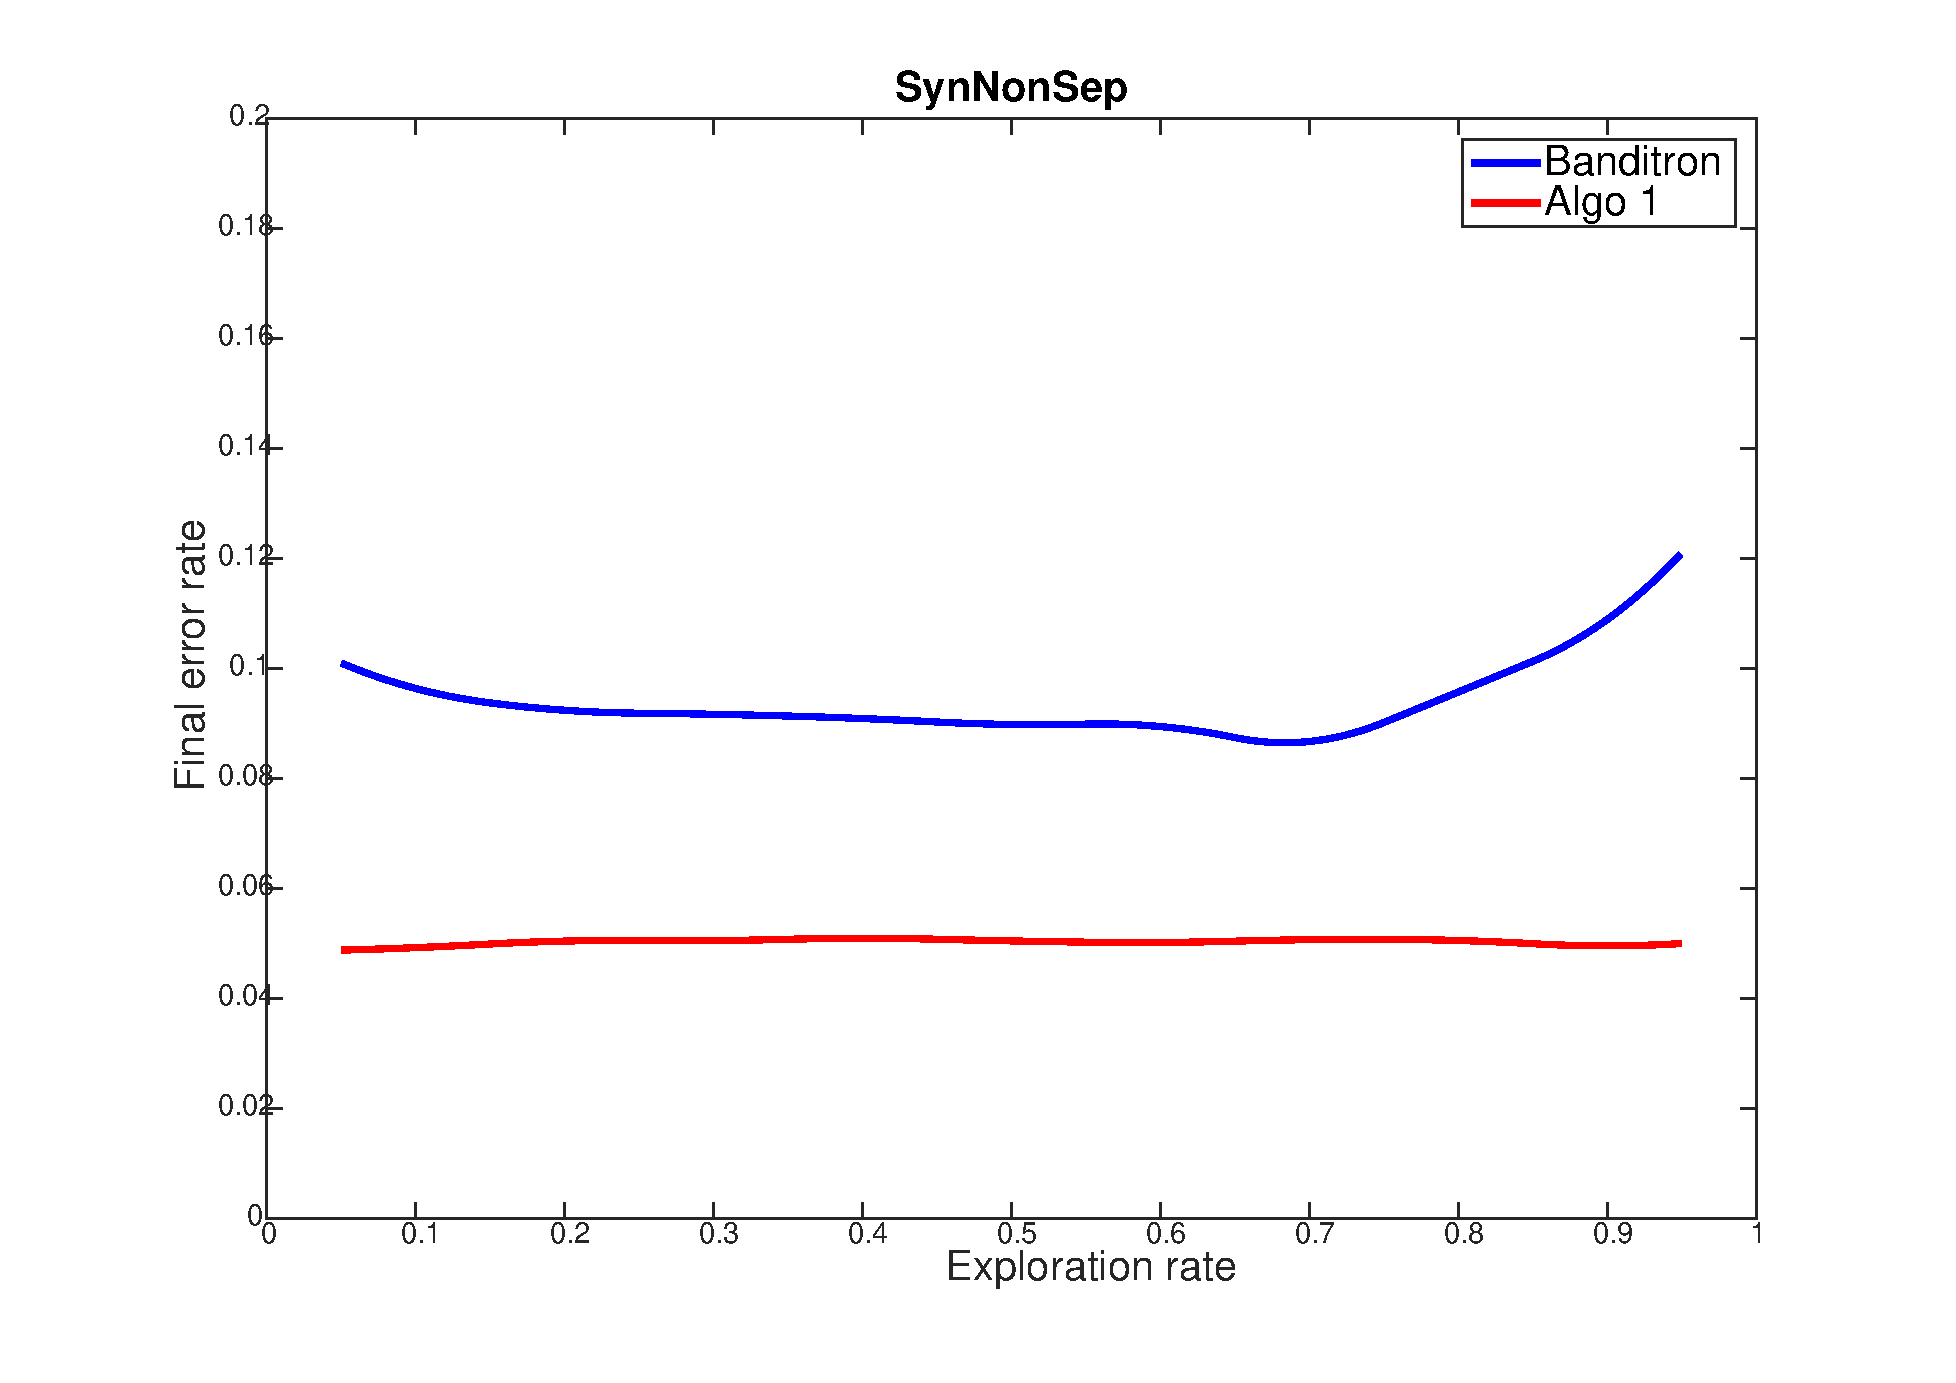
\includegraphics[scale = 0.4]{figs/SynNonSep_gamma.eps}}
	\caption{Average error of Banditron and BPA for parameter's value $\epsilon$ on the data set of SynNonSep. }
	\label{pic:BPASNSerr}
\end{figure}

\begin{figure}[h!]
	\centerline{
		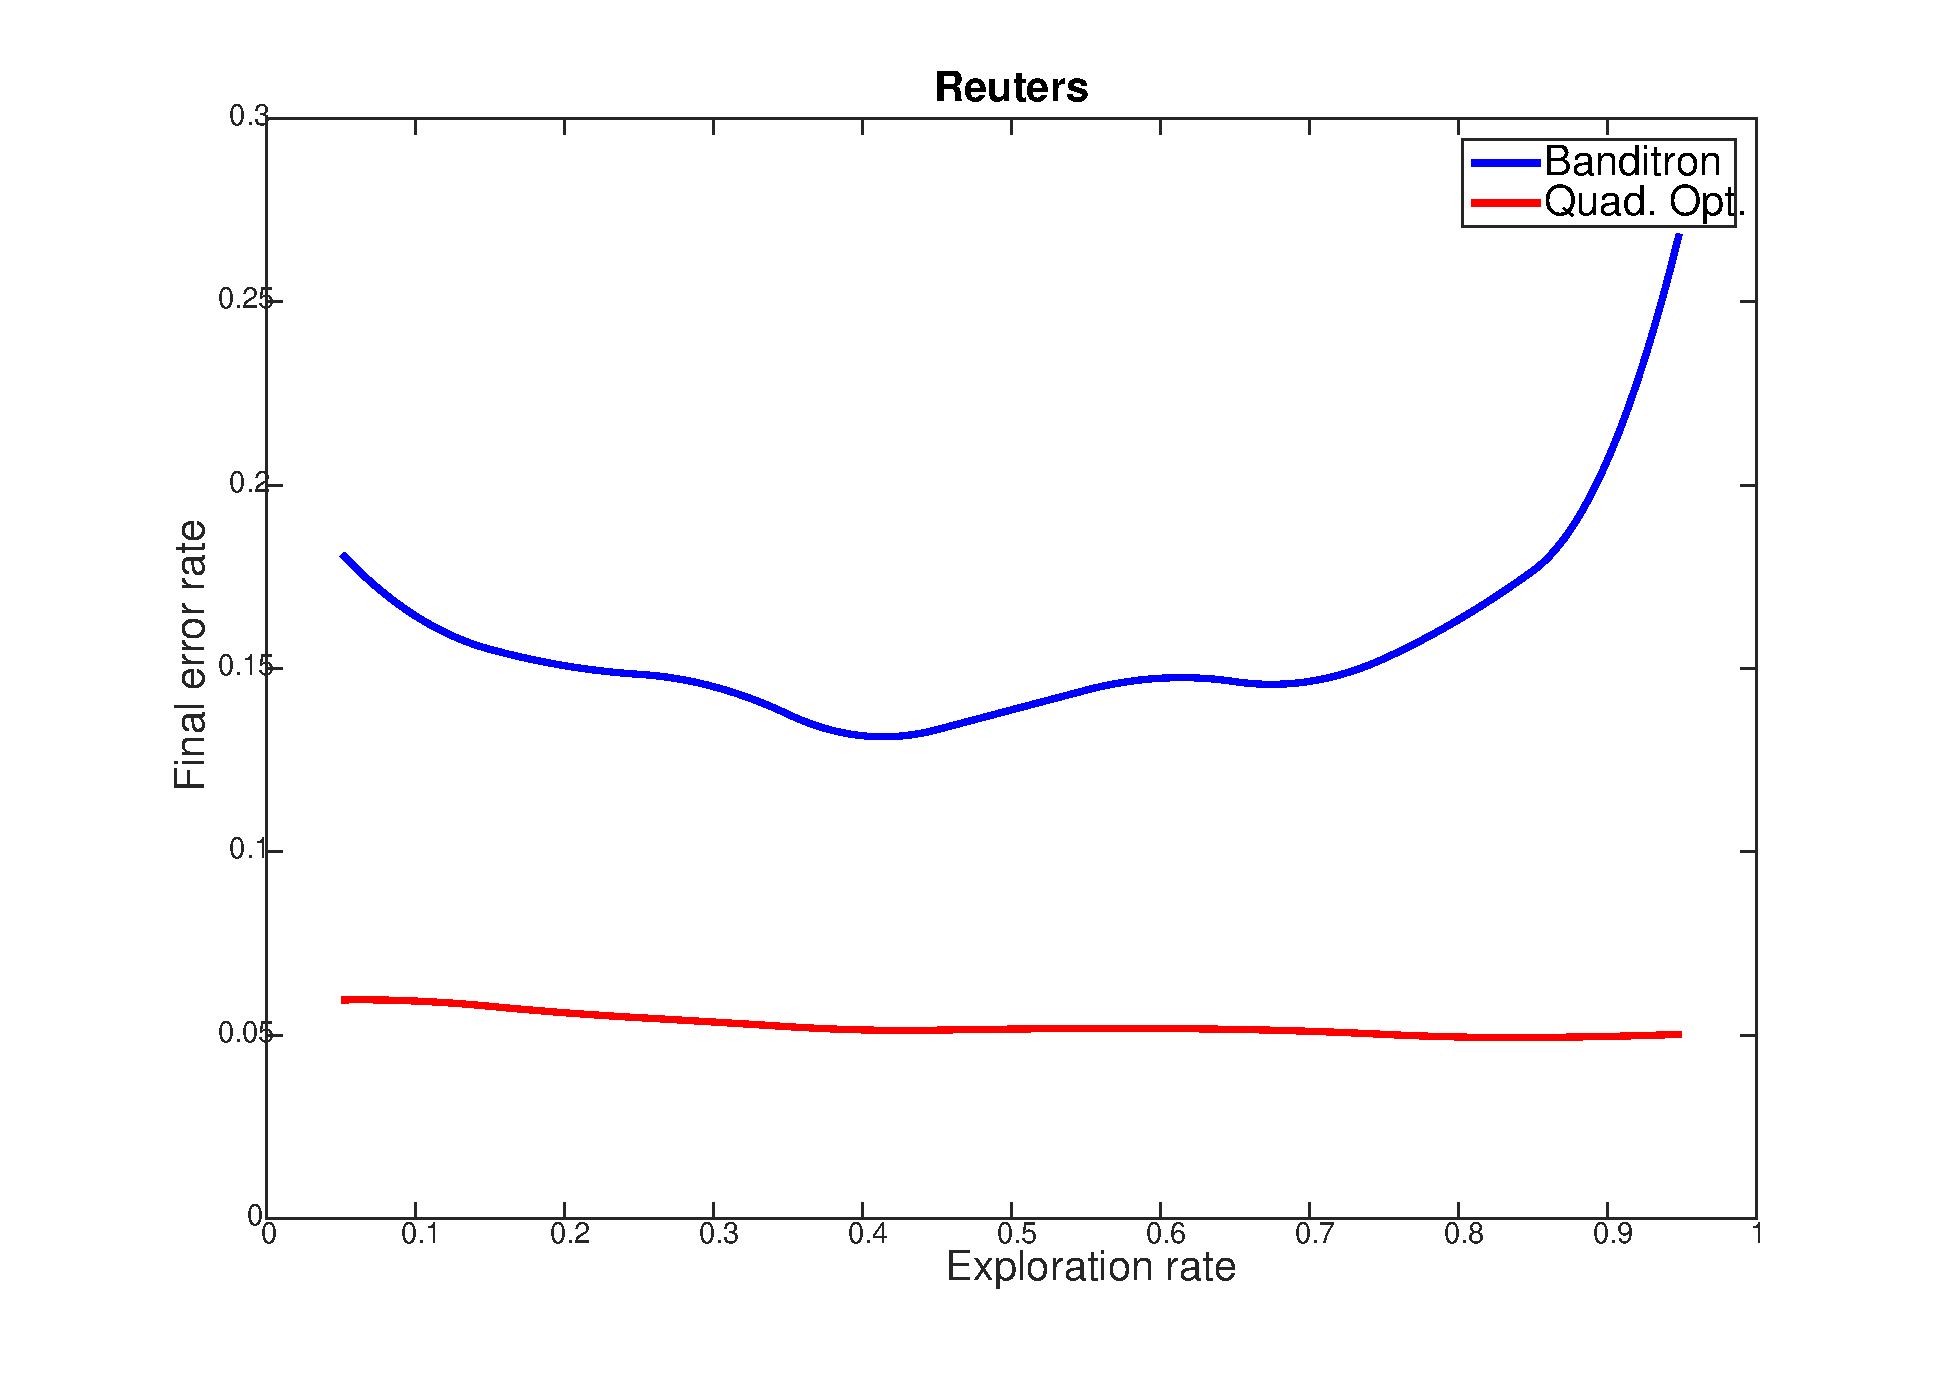
\includegraphics[scale = 0.4]{figs/Reuters_gamma.eps}}
	\caption{Average error of Banditron and BPA for parameter's value $\epsilon$ on the data set of Reuters.}
	\label{pic:BPARCVerr}
\end{figure}

\begin{figure}[h!]
	\centerline{
		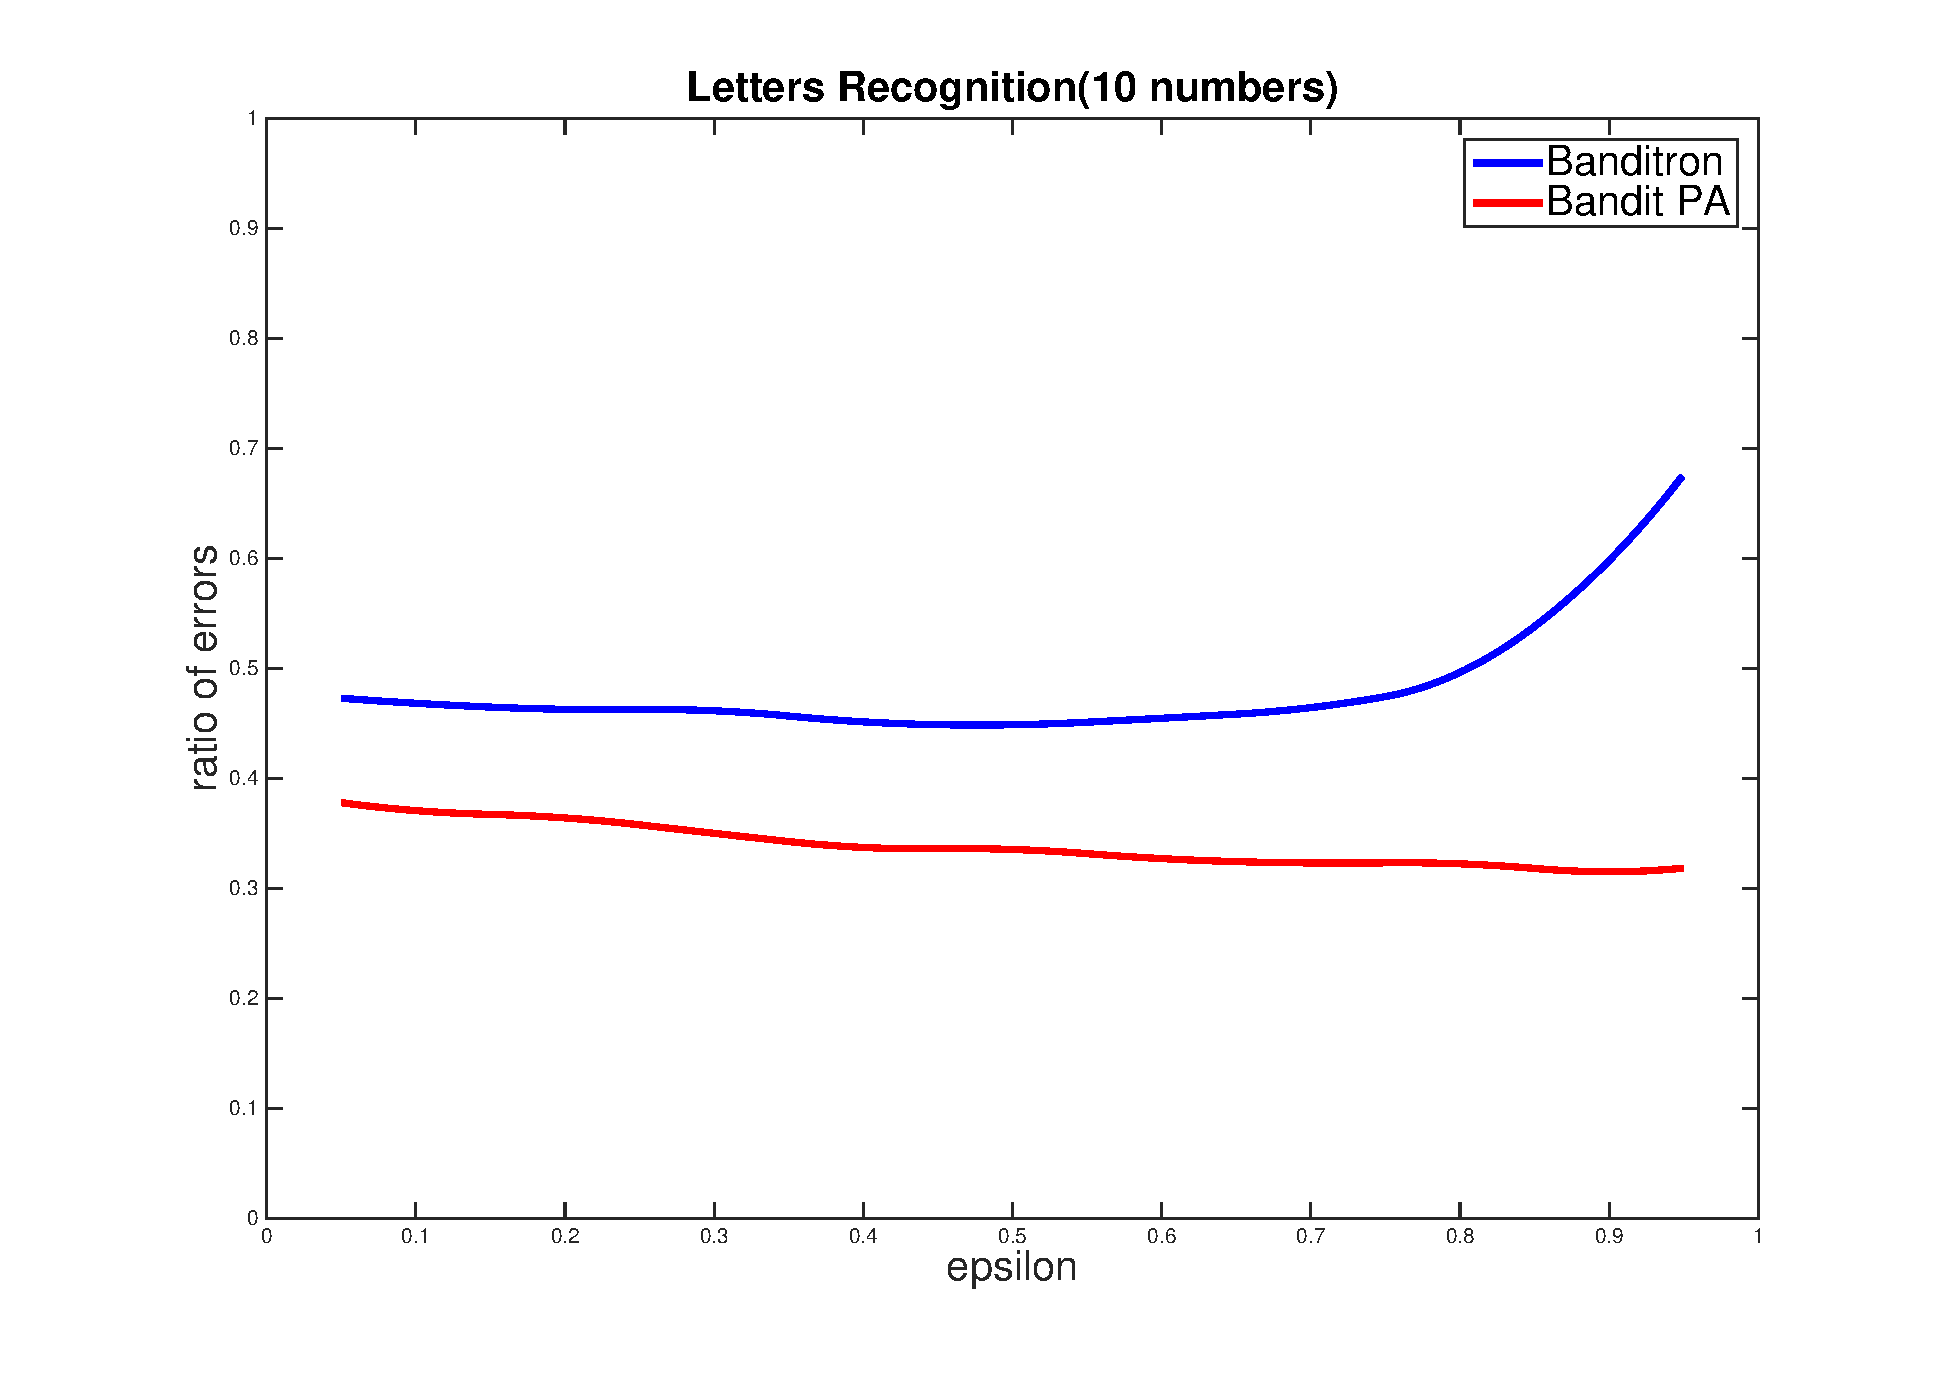
\includegraphics[scale = 0.4]{figs/10LR_gamma.eps}}
	\caption{Average error of Banditron and BPA for parameter's value $\epsilon$ on the data set of Letter Recognition.}
	\label{pic:BPALRerr}
\end{figure}


\subsection{Non-linearly separable datasets}

In this section, we take two datasets to evaluate and analyze the effect of these algorithm in Reproducing Kernel Hilbert Space.

\vspace{1.5ex}
\textbf{Data description}
The first dataset denoted by Pendigits, is a real data and created by E.Alpaydin and Fevzi.Alimoglu \cite{alimoglu1996combining,Alimoglu96methodsof}. 
It  collected 250samples from 44 writers. All writers are asked to write 250 digits in random order inside boxes of 500 by 500 tablet pixel resolution. 
Here, the dataset is part of original one. It contains 7494 instances, 16 features and 10 classes. 

The second dataset denoted by `Segment'\cite{Lichman:2013}. This dataset contains 2310 instances, all of them were drawn randomly from a database of 7 outdoor images. The images were handsegmented to create a clasification for every pixel. Each instance is a $3\times 3$ region. It's a real dataset, with 19 features and 7 classes. More details could be referred to the data site ``UCI''.

\vspace{1.5ex}
%\textcolor{red}{OK-- Il faut donner la formule des noyaux lineaire et Laplace}
\textbf{Algorithm}
Here, we take algorithms Banditron (in RKHS), KBPA and KSGD to compare. In order to perform the effect of RKHS, we choose KBPA in linear model as the reference object and choose \textbf{Laplace} for the kernel function. Its form looks like the following formulate.
\[K_{Laplace}(x,y) = \exp{\left(-\frac{\parallel{x-y}\parallel}{\sigma}\right)}\]
So, all participant algorithms contains: KBanditron, KBPA (linear), KBPA (Laplace), and KSGD (Laplace). For each dataset, the parameter of kernel function is different. By cross-validation way, we choose $\eta = 1$ of model `Laplace' for dataset Pendigits and $\eta = 10$ for dataset `Segment'. For KSGD, the truncated number is 500 for dataset Pendigits, and 200 for Segment.

\vspace{1.5ex}
\textbf{Result}
We mainly analyze these experiments from the following aspects. 

Average training time for each instance:  we observe the training time of every instance $\{t_1,t_2,\dots,t_n\}$; then divide 100 ordering examples into one group $g_1 = \{t_1,\dots,t_{100}\}$,
$\dots$, $g_i = \{t_{1+100*(i-1)},\dots, t_{100*i}\}$; finally, the average training time for instances of group $g_i$ can be calculated by $\overline{t_i} = \frac{1}{100}\sum_{s=1+100*(i-1)}^{100*i} t_s$. 

Average error rate: $e_i = \sum_{s=1+100*(i-1)}^{100\times i}\mathbf{1}_{\hat{y}_t = y_t}/100$ this measure is calculated by the same way.

Cumulative Errors: calculate the total number of past errors.

In Figure~\ref{pic:PKT}, it gives the result of average training time on based dataset ``Pendigits''.  From this result, the training time of three kernel algorithms increases linearly along with the number of training instances. Only the linear model is stable. From the theoretical perspective, Banditron always adds a new example passively for its support vector. Algorithm KSGD only adds a new example for its support vector if its classifier makes a bad prediction, otherwise the number of support vector is limited by the truncated parameter. Algorithm KBPA adds a new example for its support vector if and only if its predicted loss not equals to zero. So its number of support vector will increase all the time until it can make good prediction with no loss.

In Figure~\ref{pic:PKM} and Figure~\ref{pic:PKCM}, accumulative errors of algorithm KBPA firstly tend to a stable, others still increase linearly. That is because KBPA accumulates all good support vectors, KSGD only accumulates several recent support vectors and Kernel Banditron always accumulates new instance as negative support vector.

In Figure~\ref{pic:SKT}, it is about the average training time on dataset ``Segment''.  The training time of Kernel Banditron still increases linearly, while the training time of KSGD and KBPA are as stable as linear model after a small period of increasing linearly. KSGD reaches the limited number of support vector, and KBPA quickly gets enough support vectors to make a good prediction. It could show that this dataset is separable. 

In Figure~\ref{pic:SKM} and Figure~\ref{pic:SKCM}, we can observe that KBPA and KSGD performed obviously better than the other two.  Two kernel algorithms have ability to solve non-linear classification with Bandit Feedback. Considering the scale of classifier, we can use more efficient algorithm KBPA if dataset is separable, otherwise we use KSGD.

\begin{figure}[h!]
	\centerline{
		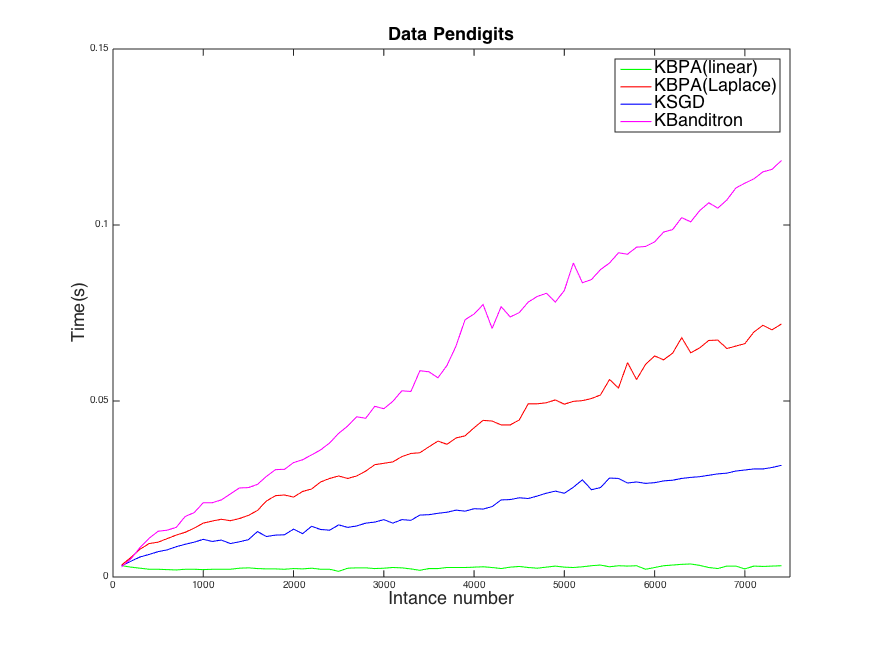
\includegraphics[scale = 0.4]{figs/Pendigits_kernel_T.png}
	}
	\caption{Average training time for each instance of Data Pendigits.}
	\label{pic:PKT}
\end{figure}

\begin{figure}[h!]
	\centerline{
		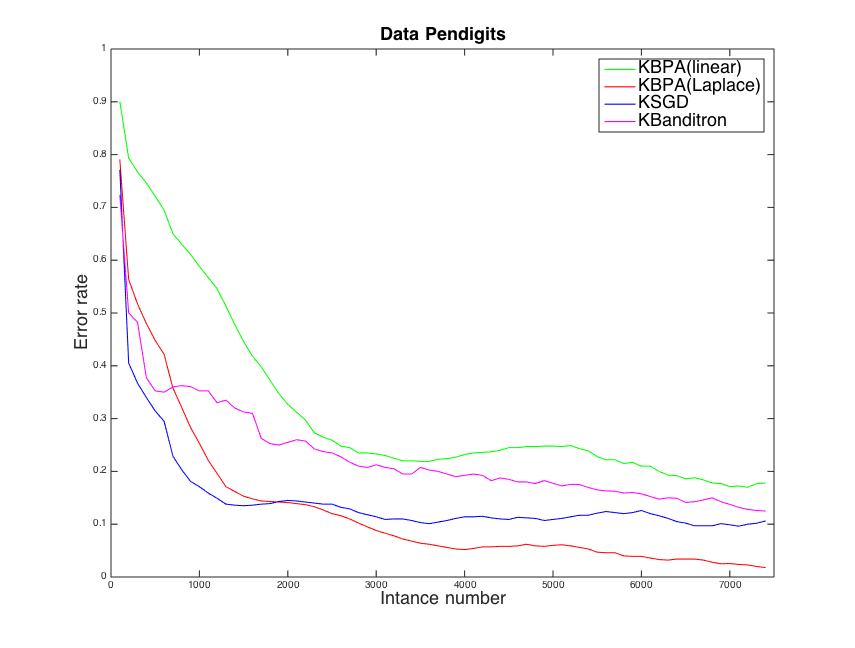
\includegraphics[scale = 0.4]{figs/Pendigits_kernel_M.png}}
	\caption{Average error rate for each instance of Data Pendigits}
	\label{pic:PKM}
\end{figure}

\begin{figure}[h!]
	\centerline{
		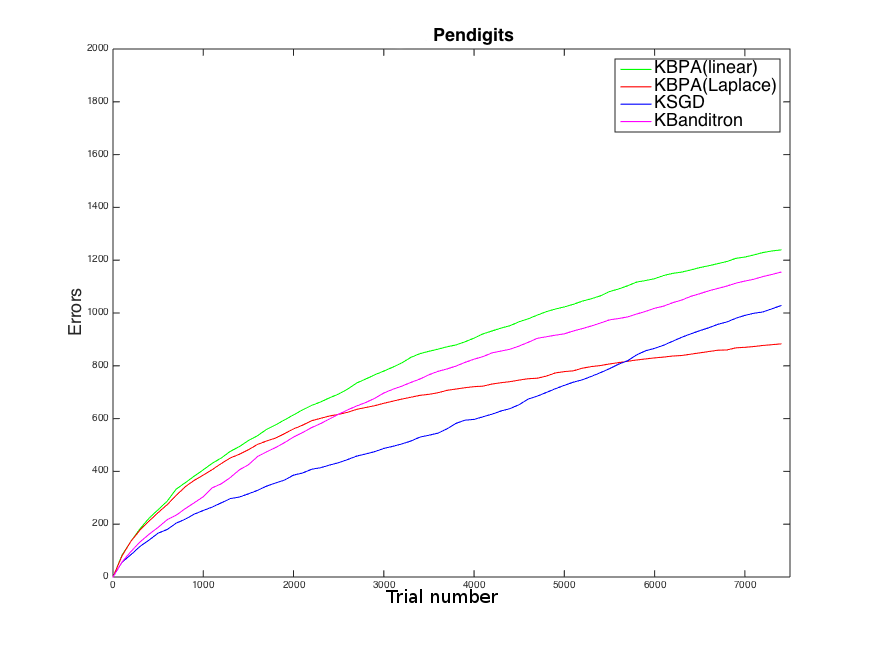
\includegraphics[scale = 0.4]{figs/Pendigits_kernel_CM.png}}
	\caption{Cumulative Errors of Data Pendigits}
	\label{pic:PKCM}
\end{figure}

%\begin{figure}[h!]
%\label{pic:PKR}
%\centerline{
%\includegraphics[scale = 0.4]{fig05/mc/Pendigits_kernel_R.png}}
%\caption{Cumulative loss of Data Pendigits}
%\end{figure}

\begin{figure}[h!]
	\centerline{
		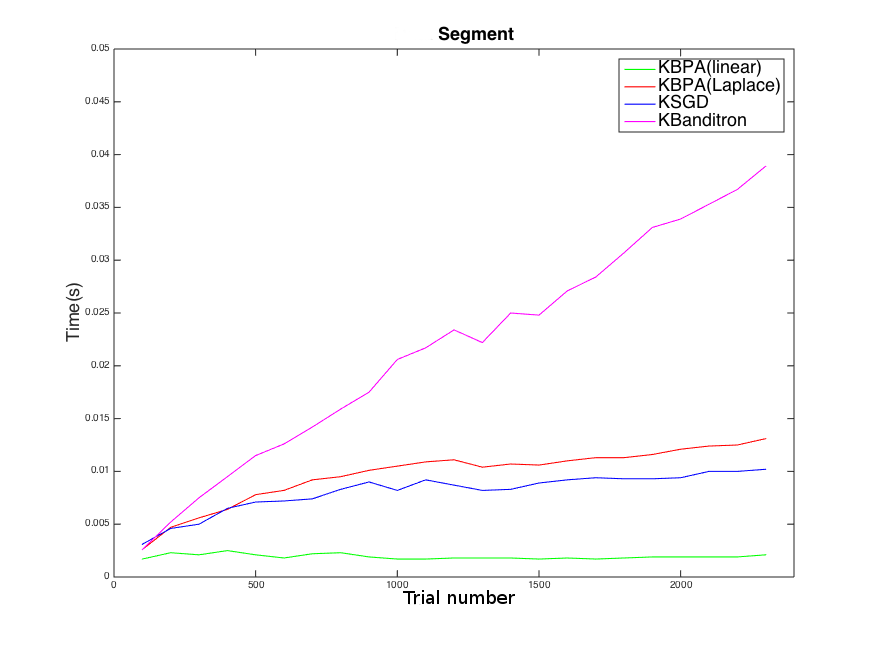
\includegraphics[scale = 0.4]{figs/Segment_kernel_T.png}}
	\caption{Average training time for each instance of Data Segment.}
	\label{pic:SKT}
\end{figure}

\begin{figure}[h!]
	\centerline{
		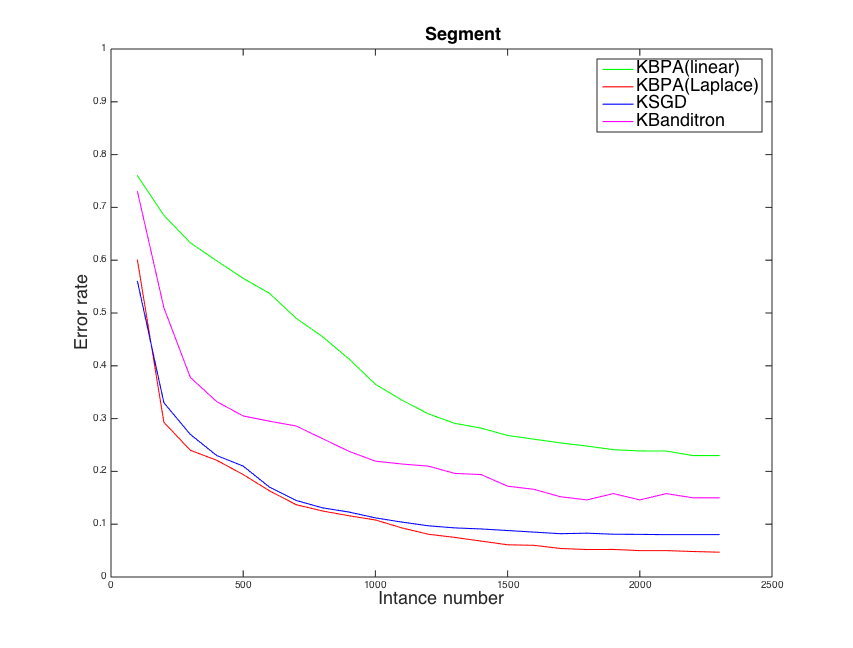
\includegraphics[scale = 0.4]{figs/Segment_kernel_M.png}}
	\caption{Average error rate for each instance of Data Segment}
	\label{pic:SKM}
\end{figure}

\begin{figure}[h!]
	\centerline{
		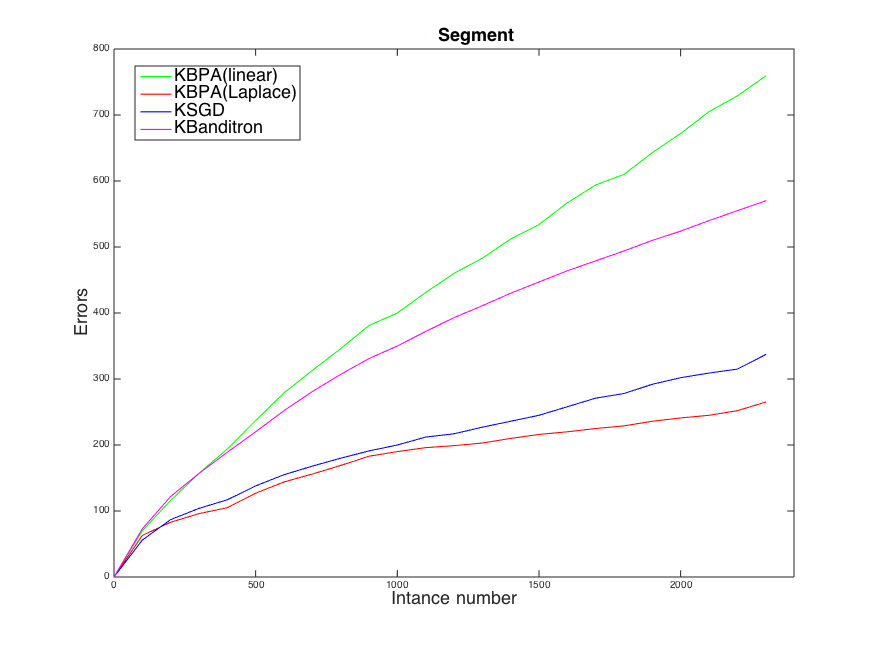
\includegraphics[scale = 0.4]{figs/Segment_kernel_CM.png}}
	\caption{Cumulative Errors of Data Segment}
	\label{pic:SKCM}
\end{figure}

%\begin{figure}[h!]
%\label{pic:SKR}
%\centerline{
%\includegraphics[scale = 0.4]{fig05/mc/Segment_kernel_R.png}}
%\caption{Cumulative loss of Data Segment}
%\end{figure}
%\subsection{Conclusion}
\section{Conclusion}
\label{sec:conclusion}
{Conclusion}
\label{subsec:BPAC}

We proposed a novel algorithm for online multiclass classification with bandit feedback. By the advantage of PA max-margin principle, BPA appears effective to address the bandit online learning setting. Its main advantage is its linear complexity in space that allows to deal with high dimensional data sets and a large number of classes, on the contrary to second-order methods. The practicability of this algorithm is verified theoretically by showing a competitive loss bound.

Moreover, experimental evaluation shows that BPA performs better than other algorithms on  real datasets, even better than the algorithms with full feedback on the data sets non-separable.

%In the next section, we will take BPA to deal with non-linear data sets  by combining the Kernel method. 



%Reading :
%Fundamental Limits of Online and Distributed Algorithms for Statistical Learning and Estimation Ohad Shamir (NIPS’14)
%Many machine learning approaches are characterized by information constraints on how they interact with the training data. These include 
%memory and sequential access constraints (e.g. fast first-order methods to solve stochastic optimization problems); 
%communication constraints (e.g. distributed learning); 
%partial access to the underlying data (e.g. missing features and multi-armed bandits) 
%algorithm with small memory footprint
%The standard implementation of many common learning tasks requires memory which is super-linear in the data dimension
%The need for fast and scalable learning algorithms has popularised the use of online algorithms, which work by sequentially going over the training data, and incrementally updating a (usually small) state vector
%There has also been considerable interest in online learning with partial information, where the learner only gets partial feedback on his performance. This has been used to model various problems in web advertising, routing and multiclass learning. Perhaps the most well-known case is the multi-armed bandits problem with many other variants being developed, such as contextual bandits, combinatorial bandits, and more general models such as partial monitoring [Bubeck, Cesa-Bianchi]
%sequential decisions


%% The Appendices part is started with the command \appendix;
%% appendix sections are then done as normal sections
%% \appendix

%% \section{}
%% \label{}

%% If you have bibdatabase file and want bibtex to generate the
%% bibitems, please use
%%
\bibliographystyle{elsarticle-harv} 
\bibliography{main}

%% else use the following coding to input the bibitems directly in the
%% TeX file.

% %\begin{thebibliography}{00}

%% \bibitem[Author(year)]{label}
%% Text of bibliographic item

%% \bibitem[ ()]{}

% %\end{thebibliography}

\end{document}

\endinput
%%
%% End of file `elsarticle-template-harv.tex'.
